\chapter{Materials and Methods}

\section{Data driven estimation of critical temperature}
\label{section:ML_models}
This part of the work was mainly inspired by the publications related to the ML-driven estimation of the critical temperature for the superconducting  \cite{Stanev:2018uk} and ferromagnetic materials \cite{Nelson:2019ui}.
In the first work \cite{Stanev:2018uk} were described several ML models for the estimation of the superconducting critical temperature over the 18000 samples dataset. The ML pipeline presented in this work consists of two models working sequentially. The first model classifies superconductors into three groups (Fe-based, cuprates, and low $T_C$ superconductors). While the second one solves the regression problem for the particular class, in other words predicting the $T_C$.  As it was reported classification models that worked solely on chemical composition information showed strong predictive power with an accuracy score of 92\%. Regression Random Forest model worked already with compositional and structural descriptors. It showed $R^2$ score of 0.85, 0.80 and 0.74 for these classes respectively

The second work \cite{Nelson:2019ui} reported the construction of several ML models in a similar way to predict the critical temperature of FM with descriptors based only on chemical composition.  The construction of proposed models did not involve any electronic structure calculations and has been entirely trained over available 2500 records of experimental data. The Random Forest algorithm gave the best-reported result with a mean absolute error (MAE) of 57 K and $R^2$ value of 0.81 over the test set containing 767 compounds. 
Also, the authors report that they made several attempts to include structural information into the descriptors. Still, such an approach did not outperform the model's predictive power containing data obtained from chemical composition only.

\subsection{Data and predictors}
The success of any ML method ultimately depends on access to reliable and plentiful data. Curie temperature data used in this work was extracted from the database provided by the authors of the described previously publication \cite{Nelson:2019ui}.  It houses 5092 experimental values of the critical temperature for ferromagnetic materials from various sources \cite{Xu2011InorganicMD,  osti_4549319}.

\subsection{Features generation}

The problem which we are working on is an estimation of Curie temperature $(T_C)$ from the sample chemical composition. It might be classified as supervised ML for the regression. The goal of supervised ML is to find a function $f(X)$ that maps the feature vector $X$, to the target variable $y(T_C)$ and allows to interpolate a set of available data to the target property in the most accurate way. In our case feature vector $(X)$ contains only the information which might be extracted from the chemical composition of a given sample. Typically, ML employs an intermediate step between compiling raw data (chemical composition) and applying a machine learning algorithm. This step converts data from a raw format into a numerical representation which is more convenient for ML algorithms and visualization. There are no rigorous rules on how it should be done, but the performance of any ML models ultimately depends on the ability to choose the most relevant descriptors.
In this work features were constructed according to the following criteria:

\begin{itemize}
\item Generation of features should not affect the size of the dataset (one should avoid the cases when descriptor could not be constructed for all the samples in dataset and missing values appears)
\item They should be easy to compute, ideally some already known properties of compounds
\item Features that allow distinguishing different materials with different chemical composition.
\end{itemize}

To accomplish this criterion were tested several existing algorithms from references \cite{Rajan:2005tl,  Rajan:2015wo,  Lookman:2016tw,  Agrawal:2016uy}, and finally made a decision to use ones described in ref.  \cite{Ward:2016va,  Ward:2018wr} employing the Materials Agnostic Platform for Informatics and Exploration (Magpie).
All produced descriptors might be divided into three groups:

\begin{enumerate}
  \item Attributes which might be determined from the periodic law: Number $(N)$, Period $(P)$, Group $(G)$, Atomic weight $(AW)$ and at some sense Mendeleev Number $(MN)$.
  \item Properties of a particular elements in a composition: Magnetic moment $(\mu)$, Bandgap $(KS)$, Melting Temperature $(T_M)$, Electronegativity $(\varepsilon)$,  Covalent radius $(R)$, lattice volume $(V)$
  \item Attributes of electronic structure, namely the fraction of electrons from the $s$, $p$, $d$, and $f$ shells
\end{enumerate}

For all categories of descriptors listed above was applied statistical functions defined below:For all categories of descriptors listed above was applied statistical functions defined below:

\begin{table}[H]

\centering
\caption{Property statistics functions}
\begin{tabular}{|p{1cm}|p{5cm}|p{5cm}|}
\hline 
N & Function & Symbol \\ 
\hline 
1 & Minimum & $x_{min}$ \\ 
2 & Maximum & $x_{max}$  \\ 
3 & Range & $\Delta x$  \\ 
4 & Mode & $\tilde{x}$ \\ 
5 & Mean & $\overline{x}$ \\ 
6 & Mean absolute deviation & $\langle x \rangle$ \\ 
\hline 
\end{tabular} 
\end{table}

For instance, property Atomic Weight $(AW)$ has features:
Minimum Atomic Weight $(AW_{min})$, maximum Atomic Weight $(AW_{max})$, range Atomic Weight $(\Delta AW)$, mode Atomic Weight $(\widetilde{AW})$, mean Atomic Weight $(\overline{AW})$, mean absolute deviation Atomic Weight $\langle AW \rangle$.

High dimensional descriptor $v_{chem} = \{ x_H, x_{He},x_{Li},x_{Be} ... \}$ describes the atomic fraction of every element in a particular sample.
For example,  \ce{Mn_2O_3} might be represented by the vector $\{ …, 0, 2/5, 0, … 0, 3/5, 0… \}$ with 3/5 assigned to the element in 8th position (Oxygen) and 2/5 to 25th (Manganese) other positions are equal to zero. The final dimensionality of generated descriptors is 215.
All the constructed descriptors presented in Table 2.

\begin{table}[H]

\centering
\caption{List of descriptors used in this work}
\begin{tabular}{|c|c|c|c|}
\hline 
N & Features & Symbol & Dim. \\ 
\hline 
1 & Atomic fraction vector & $v_{chem}$ & 90 \\ 
2 & Number & $AW_{min}$,  $AW_{max}$,  $\Delta AW$,  $\widetilde{AW}$,  $\overline{AW}$,  $\langle AW \rangle$ & 6 \\ 
3 & Period & $P_{min}$, $P_{max}$,  $\Delta P$,  $\widetilde{P}$,  $\overline{P}$,  $\langle P \rangle$ & 6 \\ 
4 & Group & $G_{min}$, $G_{max}$,  $\Delta G$,  $\widetilde{G}$,  $\overline{G}$,  $\langle G \rangle$ & 6 \\ 
5 & Mendeleev Number & $MN_{min}$, $MN_{max}$,  $\Delta MN$,  $\widetilde{MN}$,  $\overline{MN}$,  $\langle MN \rangle$ & 6 \\ 
6 & Atomic weight & $AW_{min}$, $AW_{max}$,  $\Delta AW$,  $\widetilde{AW}$,  $\overline{AW}$,  $\langle AW \rangle$ & 6 \\ 
7 & Lattice Volume & $V_{min}$, $V_{max}$,  $\Delta V$,  $\widetilde{V}$,  $\overline{V}$,  $\langle V \rangle$ & 6 \\ 
8 & Magnetic moment & $\mu_{min}$, $\mu_{max}$,  $\Delta \mu$,  $\widetilde{\mu}$,  $\overline{\mu}$,  $\langle \mu \rangle$ & 6 \\ 
9 & Bandgap & $KS_{min}$, $KS_{max}$,  $\Delta KS$,  $\widetilde{KS}$,  $\overline{KS}$,  $\langle KS \rangle$ & 6 \\ 
10 & Melting Temperature & $T^M_{min}$, $T^M_{max}$,  $\Delta T^M$,  $\widetilde{T^M}$,  $\overline{T^M}$,  $\langle T^M \rangle$ & 6 \\ 
11 & Electronegativity & $\varepsilon_{min}$, $\varepsilon_{max}$,  $\Delta \varepsilon$,  $\widetilde{\varepsilon}$,  $\overline{\varepsilon}$,  $\langle \varepsilon \rangle$ & 6 \\ 
12 & Covalent radius & $R_{min}$, $R_{max}$,  $\Delta R$,  $\widetilde{R}$,  $\overline{R}$,  $\langle R \rangle$ & 6 \\ 
13 & s-shell electrons (filled/unfilled) & $N^s_{min}$, $N^s_{max}$,  $\Delta N^s$,  $\widetilde{N^s}$,  $\overline{N^s}$,  $\langle N^s \rangle$ & 12 \\ 
14 & p-shell electrons (filled/unfilled) & $N^p_{min}$, $N^p_{max}$,  $\Delta N^p$,  $\widetilde{N^p}$,  $\overline{N^p}$,  $\langle N^p \rangle$ & 12 \\ 
15 & d-shell electrons (filled/unfilled) & $N^d_{min}$, $N^d_{max}$,  $\Delta N^d$,  $\widetilde{N^d}$,  $\overline{N^d}$,  $\langle N^d \rangle$ & 12 \\ 
16 & f-shell electrons (filled/unfilled) & $N^f_{min}$, $N^f_{max}$,  $\Delta N^f$,  $\widetilde{N^f}$,  $\overline{N^f}$,  $\langle N^f \rangle$ & 12 \\ 
\hline 
\end{tabular} 
\end{table}

\subsection{Data pre-processing}

\label{section:Data pre-processing}
Initially, the dataset contained 5092 samples. However, this data needed pre-processing since it included many compositions for which in literature was reported different values of $T_C$. There are several reasons for these occurrences. In some compounds magnetism is related to the quality of the sample, so the experiments performed by different groups and over different periods of time may report sufficiently different values of $T_C$. A second reason related to the polymorphism, namely to the existence of compounds with the same stoichiometry but different crystal structure and hence different values of $T_C$ (e.g Fe-bcc and Fe-fcc). Since at this stage the aim of this project was to construct the ML model based only on the chemical composition, structural information or details of the experiment were not included in the descriptors. In other words, feature vectors $(X)$ of two samples with the same stoichiometry are indistinguishable even thou the target property $(y)$ differs and it is not possible to extract any information about polymorphism or sample quality.
As such it was made a decision to establish criteria to exact a single value of $T_C$ for the samples with the same stoichiometry. In this work was used the median of the distribution instead of mean or maximum value since it is less dependent on the possible outliers. For example, if for the same stoichiometry was reported 3 different values of $T_C$ 305, 330, and 600K they were replaced with a single median value of $T_C = 330 K$. Of course, such an approach has drawbacks. In cases when we have an even number of samples with the same stoichiometries (e.g. 4 or 6) $T_C$ also depends on a half sum of the distribution central values. But after all, it allows us to operate with more reliable values since most of them are associated with real experimental measurements but not with a mean value of several experiments. After this operation, the size of the dataset decreased almost by half and became 2557 samples, which might be considered as relatively small from the point of view of ML algorithms. Distribution of $T_C$ temperatures in the pre-processed data shown on Figure \ref{fig:tc_distrib}.

\begin{figure}[H]
	\centering
	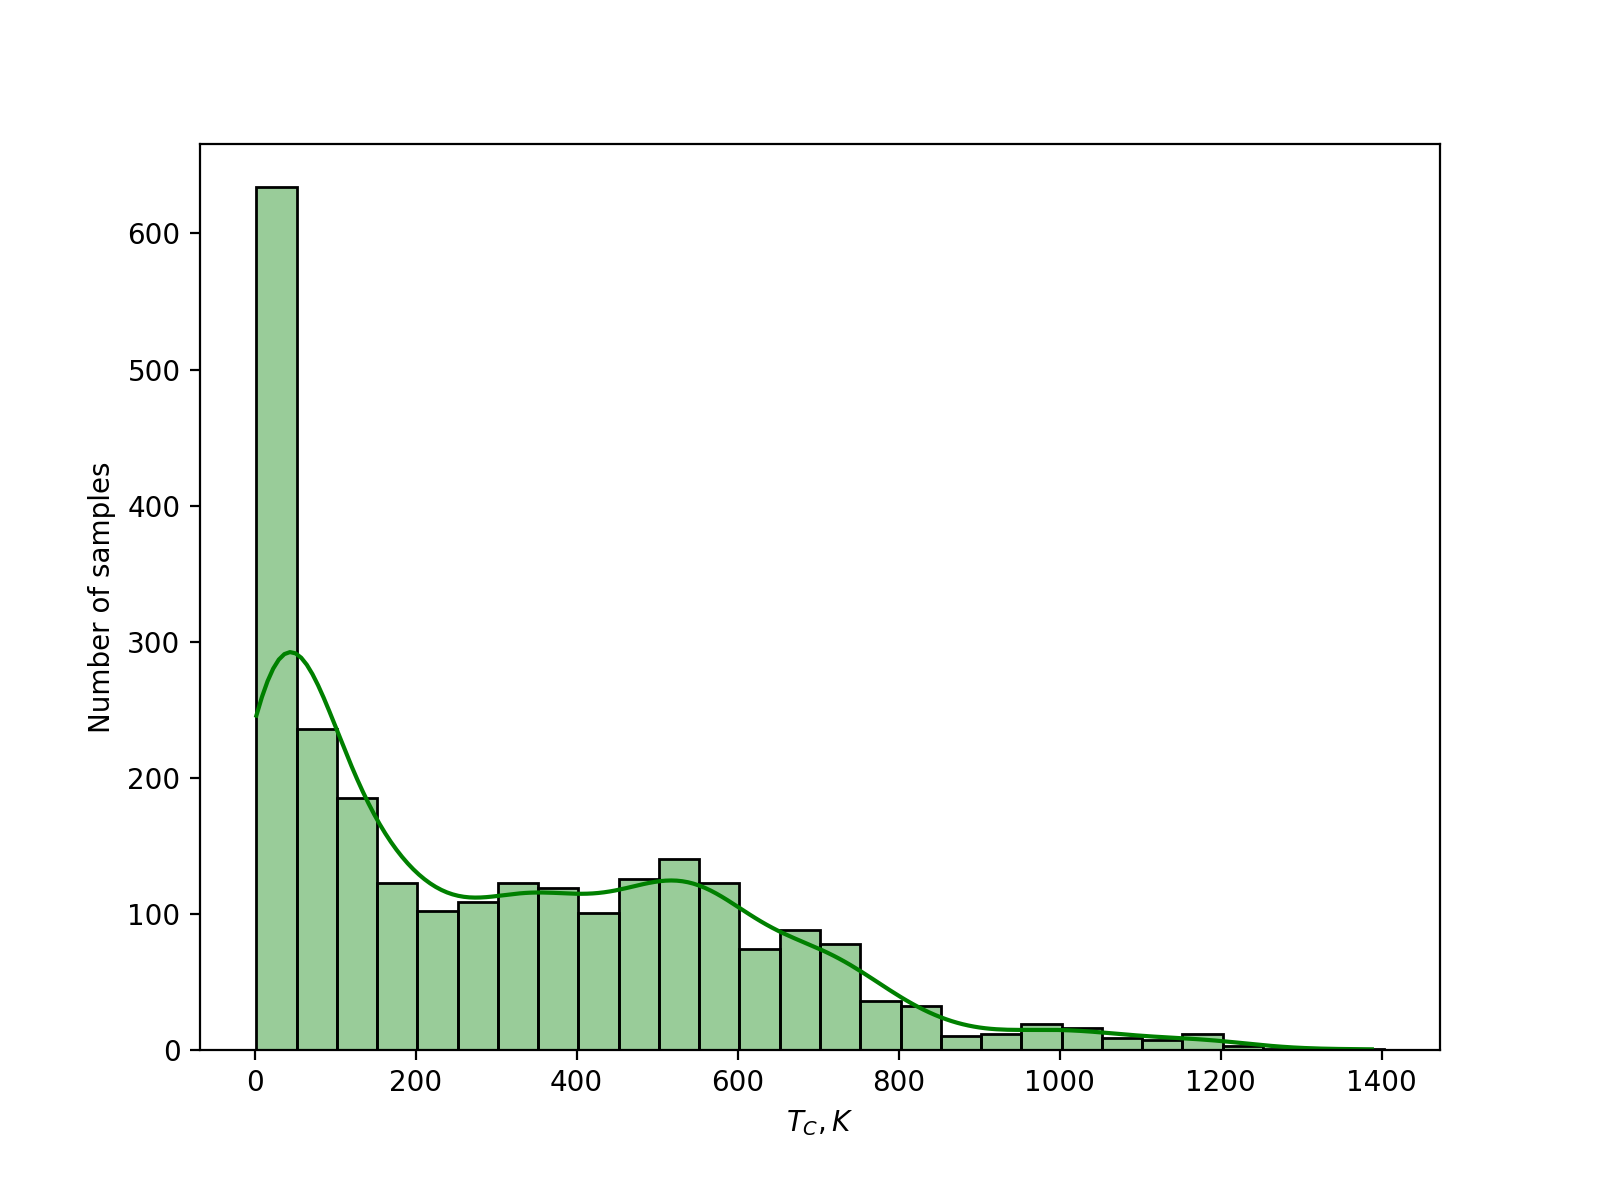
\includegraphics[width=160mm]{fig/ml_fig/tc_distrib.png}
	\caption[Critical temperature distribution histogram over 2557 samples]{Distribution of critical temperature over 2557 samples.}
\label{fig:tc_distrib}
\end{figure}

\subsection{Machine-learning models}

\subsubsection{Models evaluation}

As it was already mentioned the size of our data is relatively small. This fact means that we were not able to follow the standard procedure of the model training and evaluation which requires splitting of the data into three equal and mutually exclusive partitions namely training, testing, and validation sets. In case when the dataset is not so big such split makes each of the subsets too small decreasing the overall ability to learn and thus accuracy. That’s why the entire dataset was divided only into 2 not equal parts: 1st is a training set which included 2/3 of the data (1714 samples) and 2nd is testing set consisting of the remaining 834 samples. Schematically this process shown in Figure \ref{fig:ml_model_eval}.

\begin{figure}[H]
\centering
\captionsetup{justification=centering,margin=2cm}
	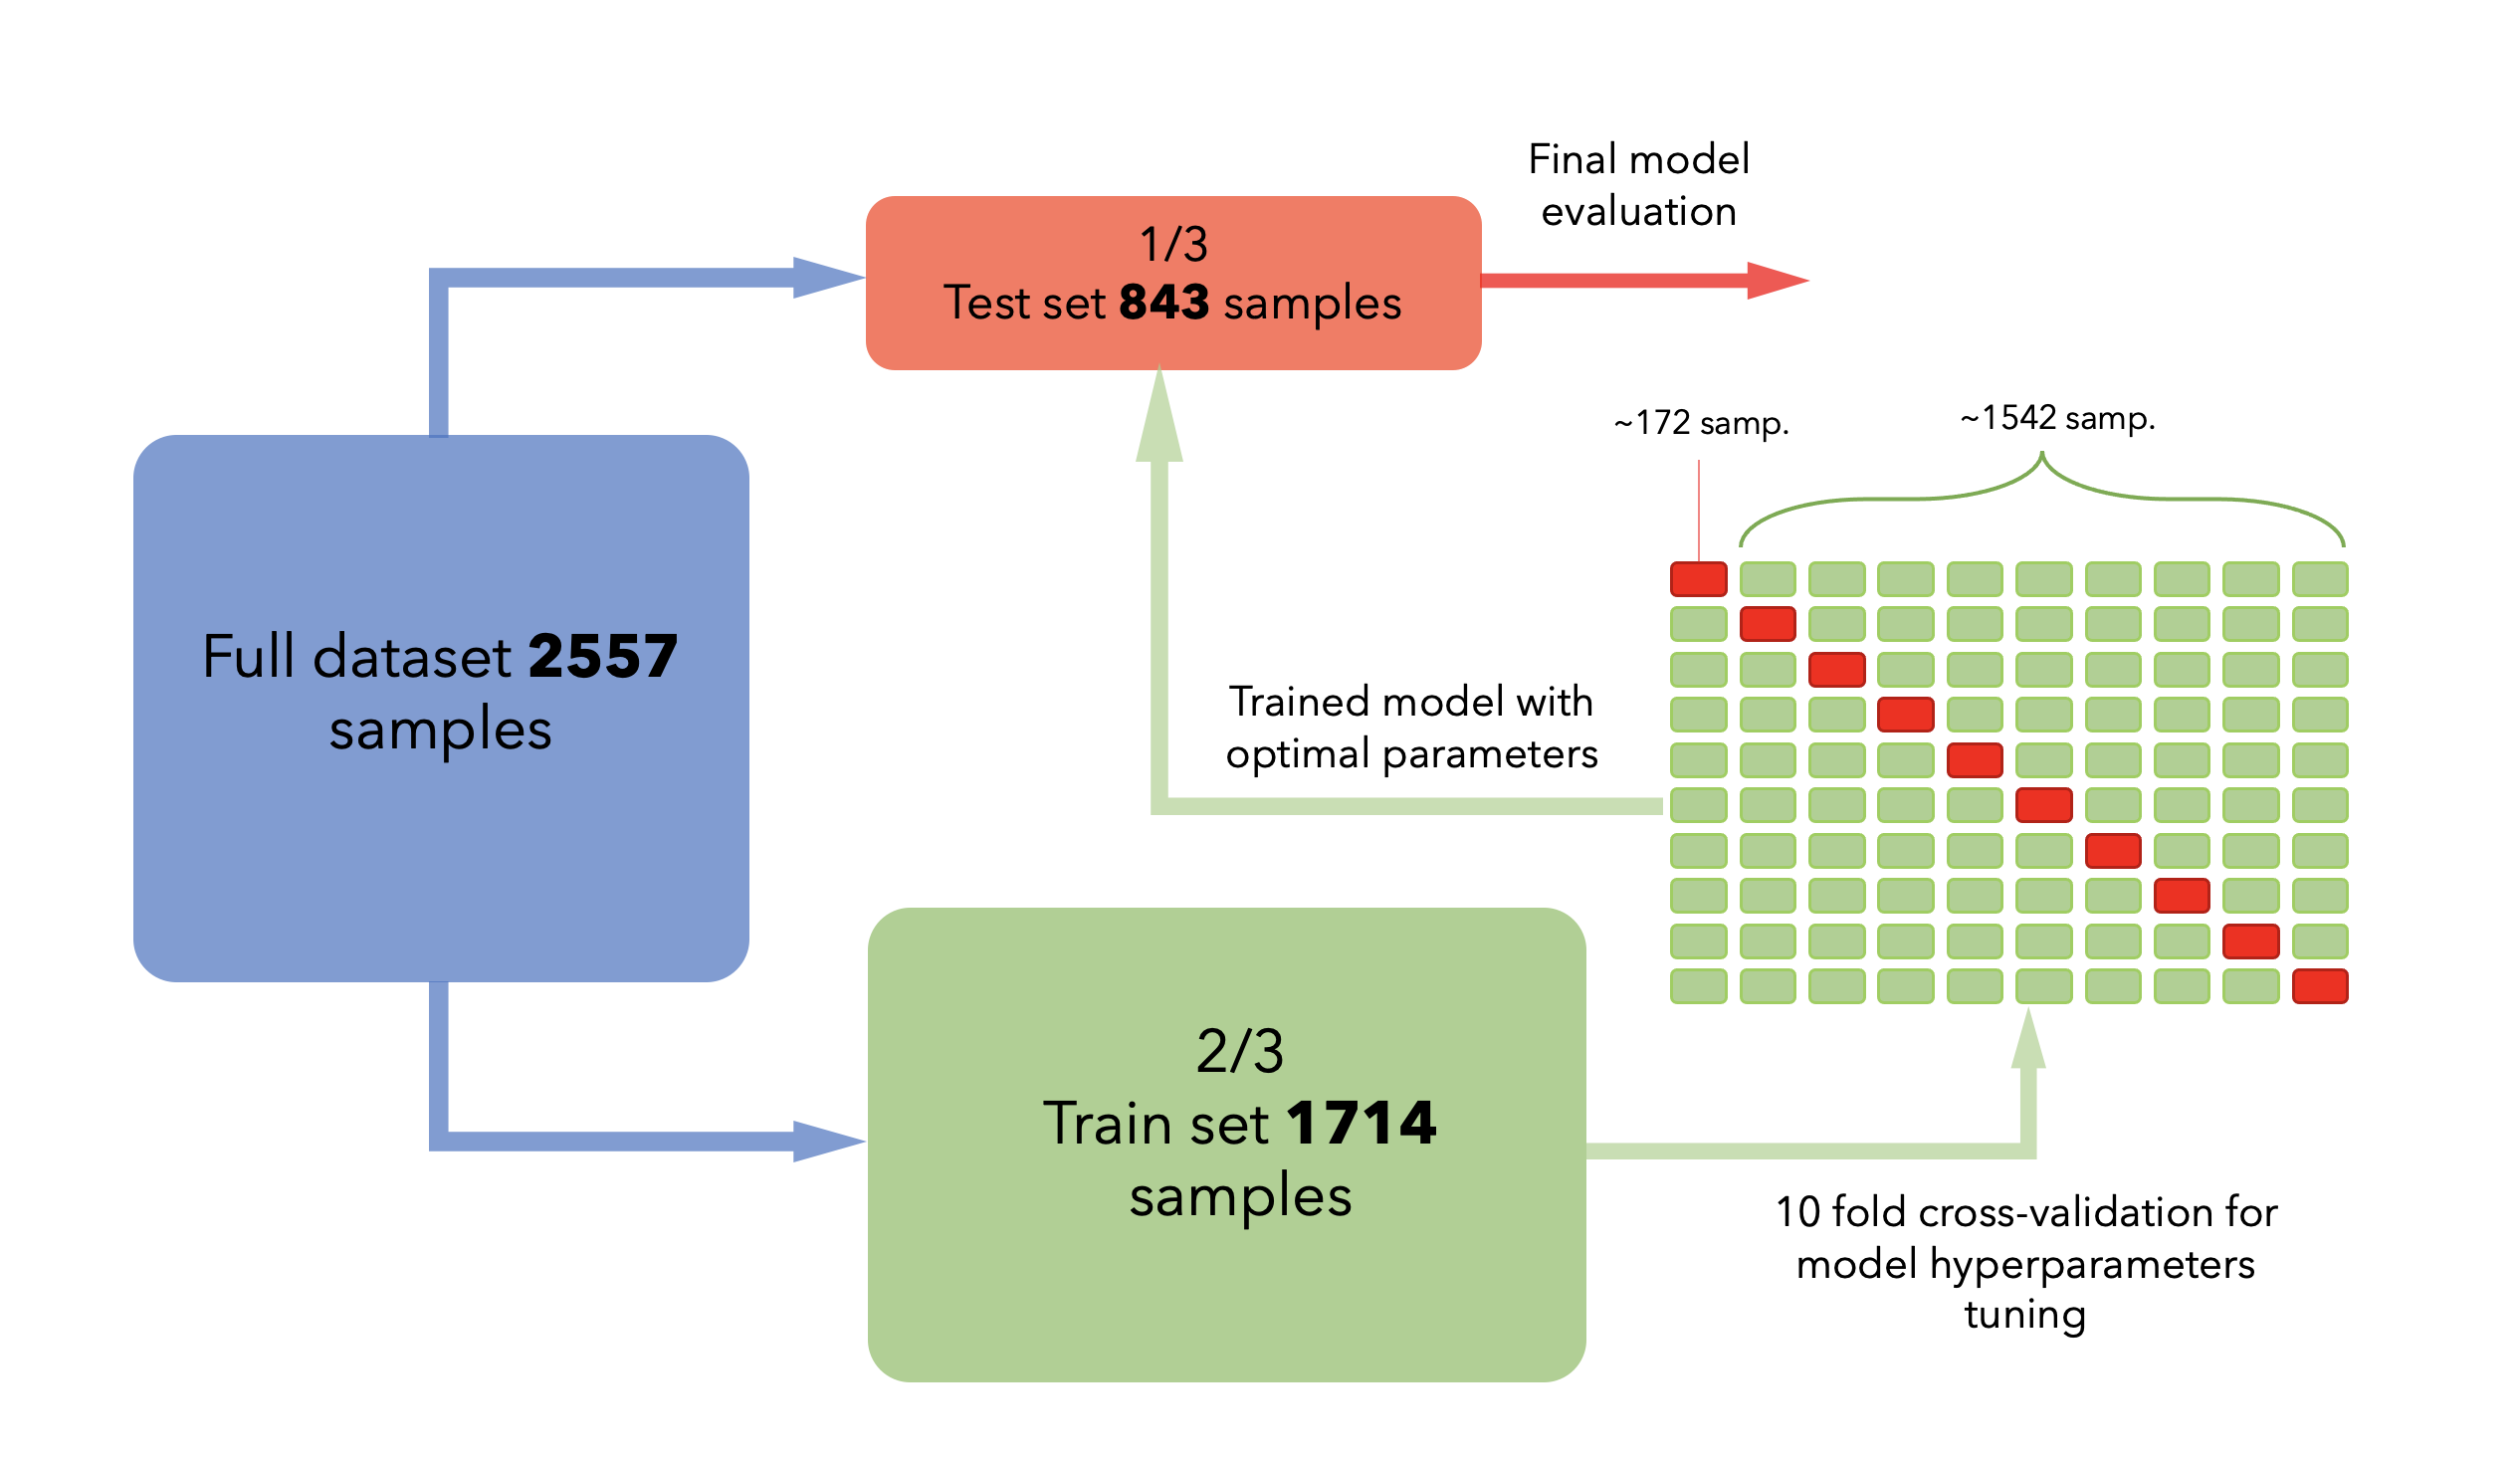
\includegraphics[width=160mm]{fig/ml_fig/model_eval.png}
	\caption[Scheme of cross-validation process followed by final model evaluation on the test subset.]{Scheme of cross-validation process followed by final model evaluation on the test subset.}
\label{fig:ml_model_eval}
\end{figure}

Hyperparameters optimization for all models was performed through the standard K-fold cross-validation procedure. The training set is split into K subsets (in this work K=10) then the model is trained over the K-1 sets and evaluated on the remaining one, thus the cross-validation error is an average error of the K evaluation rounds. The best model (model with optimum hyperparameters) is a model with the lowest cross-validation error.
Finally, the test set was used for estimation the generalization error of the model, namely for assessing how well the given model performs on never-seen-before data.

Quantitively model’s performance were measured by the coefficient of determination $R^2$:

\begin{equation}
R^2 = 1 - \frac{\sum \limits_{i}( y_i - f(x_i))^2}{\sum \limits_{i} (y_i - \mu)^2}
\end{equation}

and root mean squared error (RMSE):

\begin{equation}
RMSE = \sqrt[]{\frac{\sum \limits_{i}( y_i - f(x_i))^2}{n}}
\end{equation}

Here: $y_i$ - target property; $f(x_i)$ - predicted value; $\mu$ - mean

For the perfect predictor, namely $y_i = f(x_i)$, these values should be equal to 1 and 0 respectively.
$RMSE$ and $R^2$ were specified as the main optimization parameters for all trained models. Also, for the all models were estimated and reported maximum error but this parameter was not chosen as an optimization one.
In the constriction of ML models were compared four different algorithms:
\begin{enumerate}
\item Kernel Ridge Regression (KRR)
\item Random Forest (RF)
\item Extreme Gradient Bosting (XGBoost)
\item Sure Independence Screening plus Sparsifying Operator (SISSO)
\end{enumerate}

The first three models come from Python distributions Scikit-Learn \cite{Pedregosa:2012tv} and XGBoost \cite{Chen_2016} respectively. SISSO is a separate algorithm on Fortran 90 \cite{Ouyang_2018, Ouyang_2019}. KRR, RF, and XGBoost were trained and evaluated following the 10-fold cross-validation and testing procedure described previously. SISSO was trained on entire dataset without accurate validation, due to the lack of computational resources. Hyperparameters tuning for every model will be described explicitly.

\subsubsection{Kernel ridge regression.}
The first model which was chosen as a baseline for particular work is a Kernel Ridge Regression (KRR). Simple Ridge Regression was not considered since the sufficiently large dimensionality of the descriptors might significantly affect the performance of this model.
Kernel ridge regression combines ridge regression (linear least squares with $l_2$-norm regularization) with the kernel trick. Which in compare to Ridge Regression might be written as follows:
Ridge regression:
\begin{equation}
y = w^T\phi(x)
\end{equation}

The idea is to minimize loss function (estimate the best weights):

\begin{equation}
J(w) = \sum \limits_{i=1}^{n}(y_n-w^Tx_n)^2
\end{equation}

Not kernilized solution of this equation for the nonlinear regression might be written as follows:

\begin{equation}
w = (\phi^T\phi+\lambda I)^{-1}\phi^Ty
\end{equation}

Kernel Trick allows as to sufficiently decrease the complexity of this solution, since the dot product $\phi\phi^T$ can be found just as $K(x_m,x_n)$ function:

\begin{equation}
w = (\phi^T(\phi\phi^T+ \lambda I))^{-1} y
\end{equation}

\begin{equation}
K(x_m,x_n) = \phi \phi ^ T
\end{equation}

It thus learns a linear function in the space induced by the respective kernel and the data. For non-linear kernels, this corresponds to a non-linear function in the original space.
In this work KRR algorithm was tuned with respect to the regularization parameter $\lambda$ and different Kernels, namely:

\begin{align}
&K(x_m,x_n) = x_m^T x_n\\
&K(x_m,x_n) = (x_m^T x_n + r) ^ d \\
&K(x_m,x_n) = \exp \left(- \frac{|| x_m - x_n || ^ 2}{2\sigma} \right)\\
&K(x_m,x_n) = \exp \left( -\alpha ||x_m - x_n || ^ 2 \right)
\end{align}


It turns out that for all non-linear Kernels optimal value of optimization parameter $\lambda$ is equal to 0.10 (tested in range 0.05 - 1). 
Best $R^2$ and $RMSE$ scores were achieved by the Laplacian Kernel which is also the most computationally demanding one (required almost 5 times more computational resources than others). 
The lowest value of maximum error was given by the simplest linear Kernel.
Performance of different KRR models shown on scatter plots in Figure \ref{fig:krr_results}, and also in table \ref{tab:krr_results}.

\begin{table}[H]
\centering
\caption{KRR models performance with respect to different Kernels}
\begin{tabular}{|p{3cm}|p{2.5cm}|p{2.5cm}|p{2.5cm}|p{2.5cm}|}
\hline 
Metrics/Kernel & Linear & Polynomial & RBF & Laplacian \\ 
\hline 
R2 (test) & 0.616
 & 0.759 & 0.756 & 0.793 \\ 
R2 (cross.val) & 0.601 & 0.768 & 0.754 & 0.787 \\ 
RMSE (K) & 161.9 & 
131.4 & 132.3 & 121.7 \\ 
Max Error (K) & 598.1 & 783.4 & 795.6 & 642.05 \\ 
\hline 
\end{tabular} 
\label{tab:krr_results}
\end{table}

\begin{figure}[H]
\centering
\captionsetup{justification=centering,margin=2cm}
	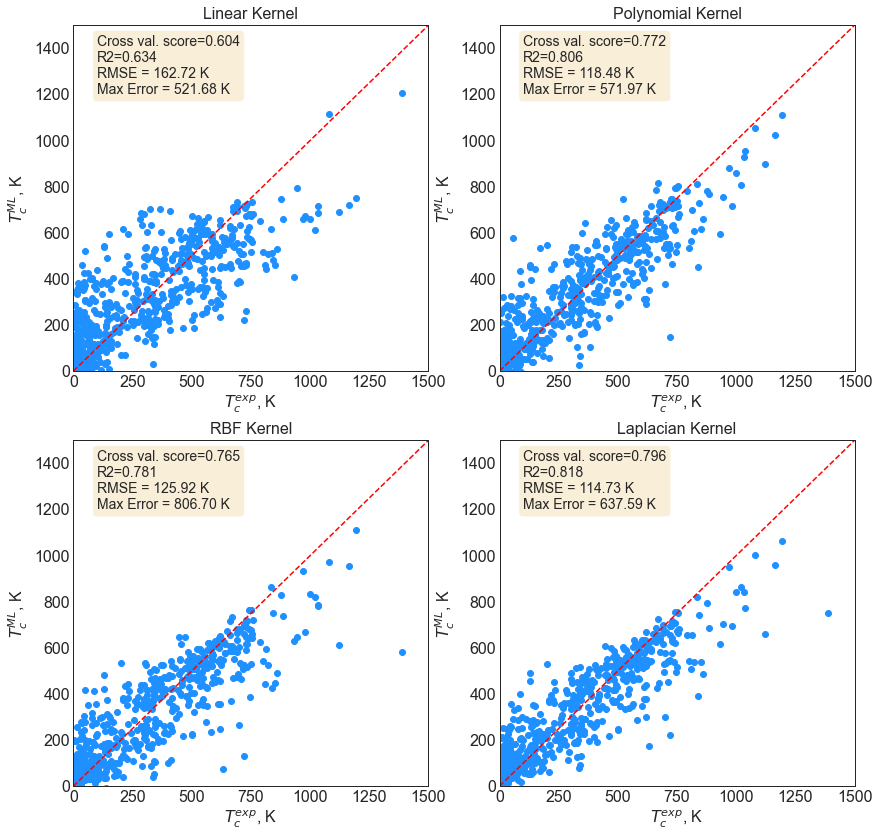
\includegraphics[width=160mm]{fig/ml_fig/krr_results.png}
	\caption[Comparison of experimental and predicted values of Curie temperature for different Kernels.]{Comparison of experimental $(T_C^{exp})$ and predicted values $(T_C^{ML})$ for different Kernels.}
\label{fig:krr_results}
\end{figure}



\subsubsection{Random forest algorithm}

Random forest (RF) is one of the most powerful, versatile, and widely used ML methods. RF, like its name implies, consists of a large number of individual decision trees (see Figure \ref{fig:rf_scetch}) that operate as an ensemble. Each individual tree in the RF trains only on a random part of the training set samples and also only on the randomly selected subspace of descriptors (i.e. every tree in RF learns on different samples and features). This approach allows to build a large number of relatively uncorrelated models (trees) which operating as a committee will outperform any of the individual constituent models.

\begin{figure}[H]
	\centering
	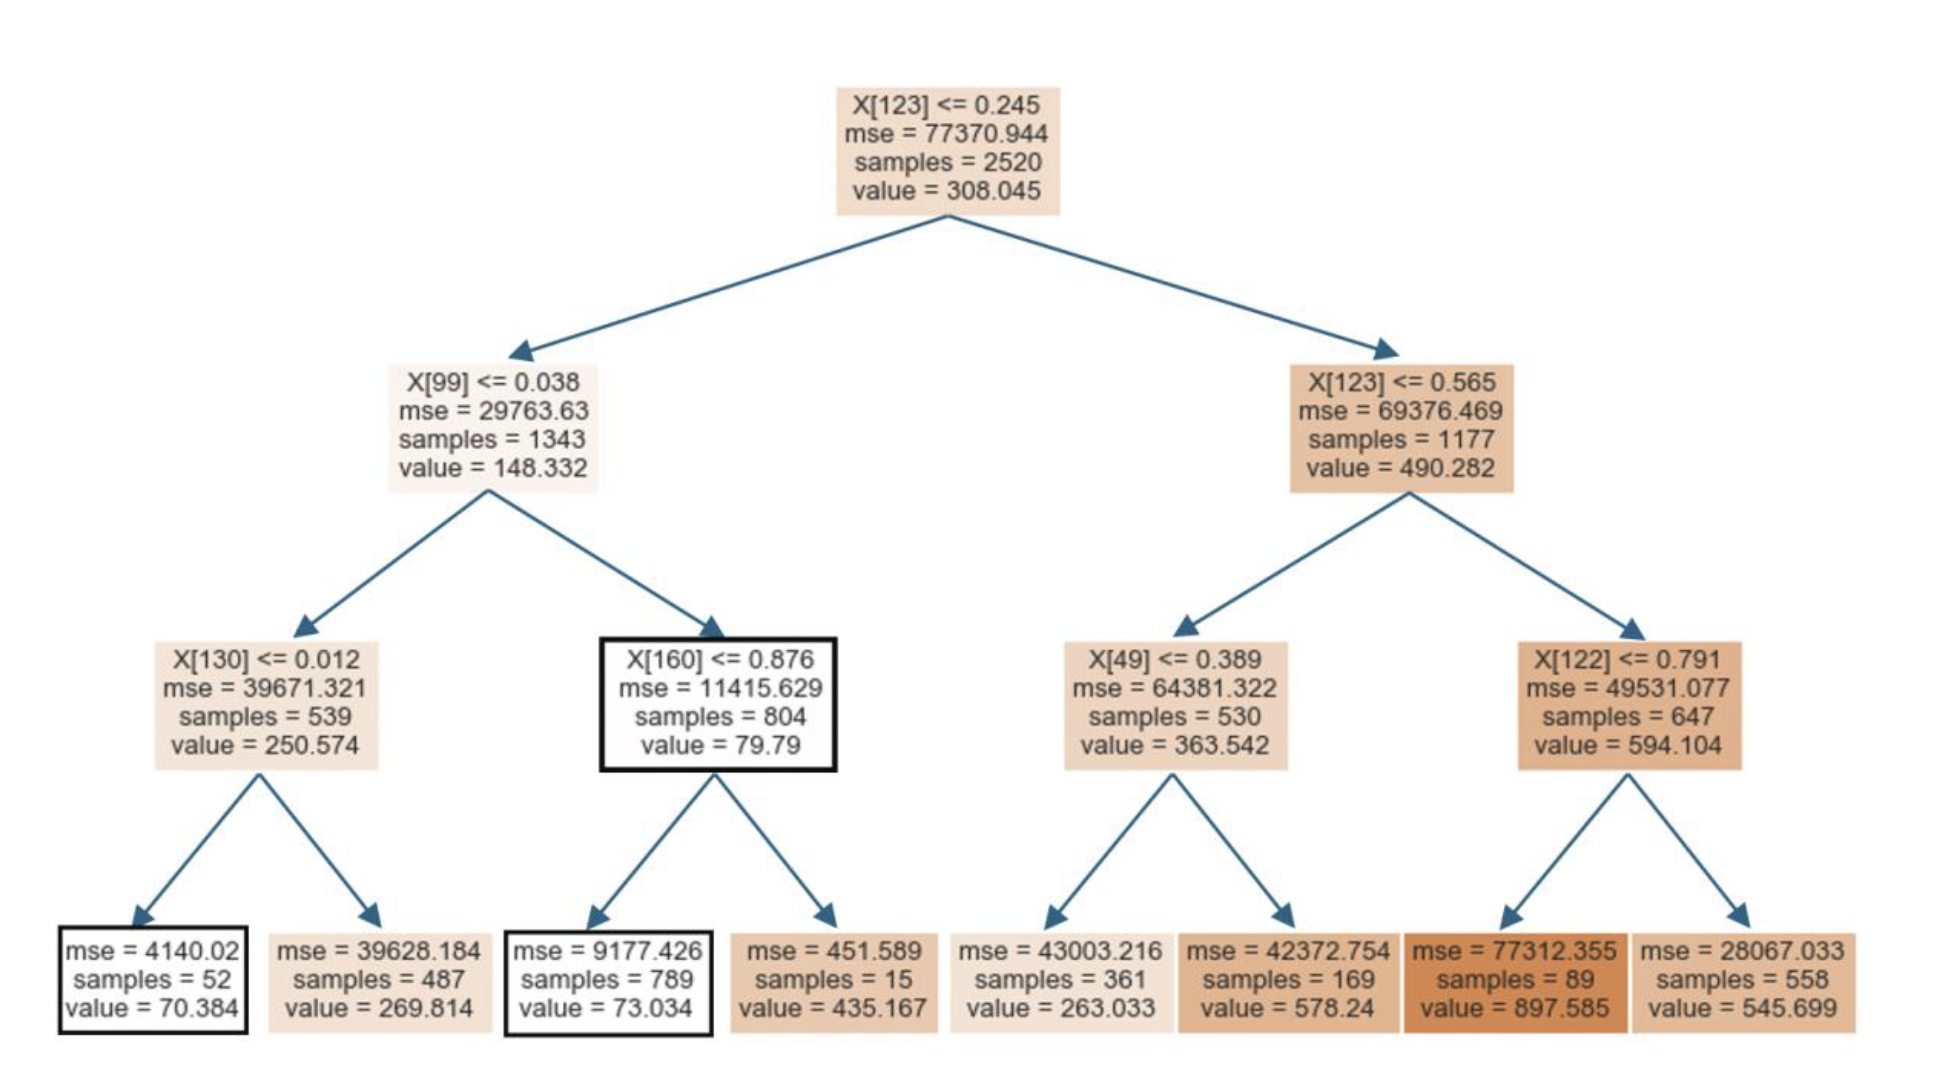
\includegraphics[width=140mm]{fig/ml_fig/rf_scetch.png}
	\caption[Single Tree model with depth 4 for the regression problem under consideration.]{Single Tree model with depth 4 for the regression problem under consideration.}
\label{fig:rf_scetch}
\end{figure}

There are several important advantages that make it especially suitable for the problem under consideration. First, it can find complicated non-linear dependencies from the data. Compare to the number of other methods (e.g. linear regression), it does not make any assumptions or fitting about the functional form of the relationship between the predictors and the target variable. The second important advantage of this method is that, by combining information from individual independent predictors (trees), it can determine the importance of each particular feature, thus making the whole model more interpretable, and allows us to extract useful insights from the trained model.
For example, predictor importance was employed for the decreasing of the feature space dimensionality. Predictors were sorted according to their importance and firstly were removed 25\% of less important features (Q75) and then another 25\% (Q50). New models were trained and evaluated on the reduced features spaces (Q50, Q75) as it is shown in Table \ref{tab:rf_results}.
Hyperparameters that were optimized are maximum tree depth as shown in Figure \ref{fig:rf_convergence} (a) and the number of trees Figure \ref{fig:rf_convergence}(b). Convergence was achieved after 100 trees in an ensemble with a depth equal to 10.

\begin{figure}[H]
\centering
\captionsetup{justification=centering,margin=2cm}
	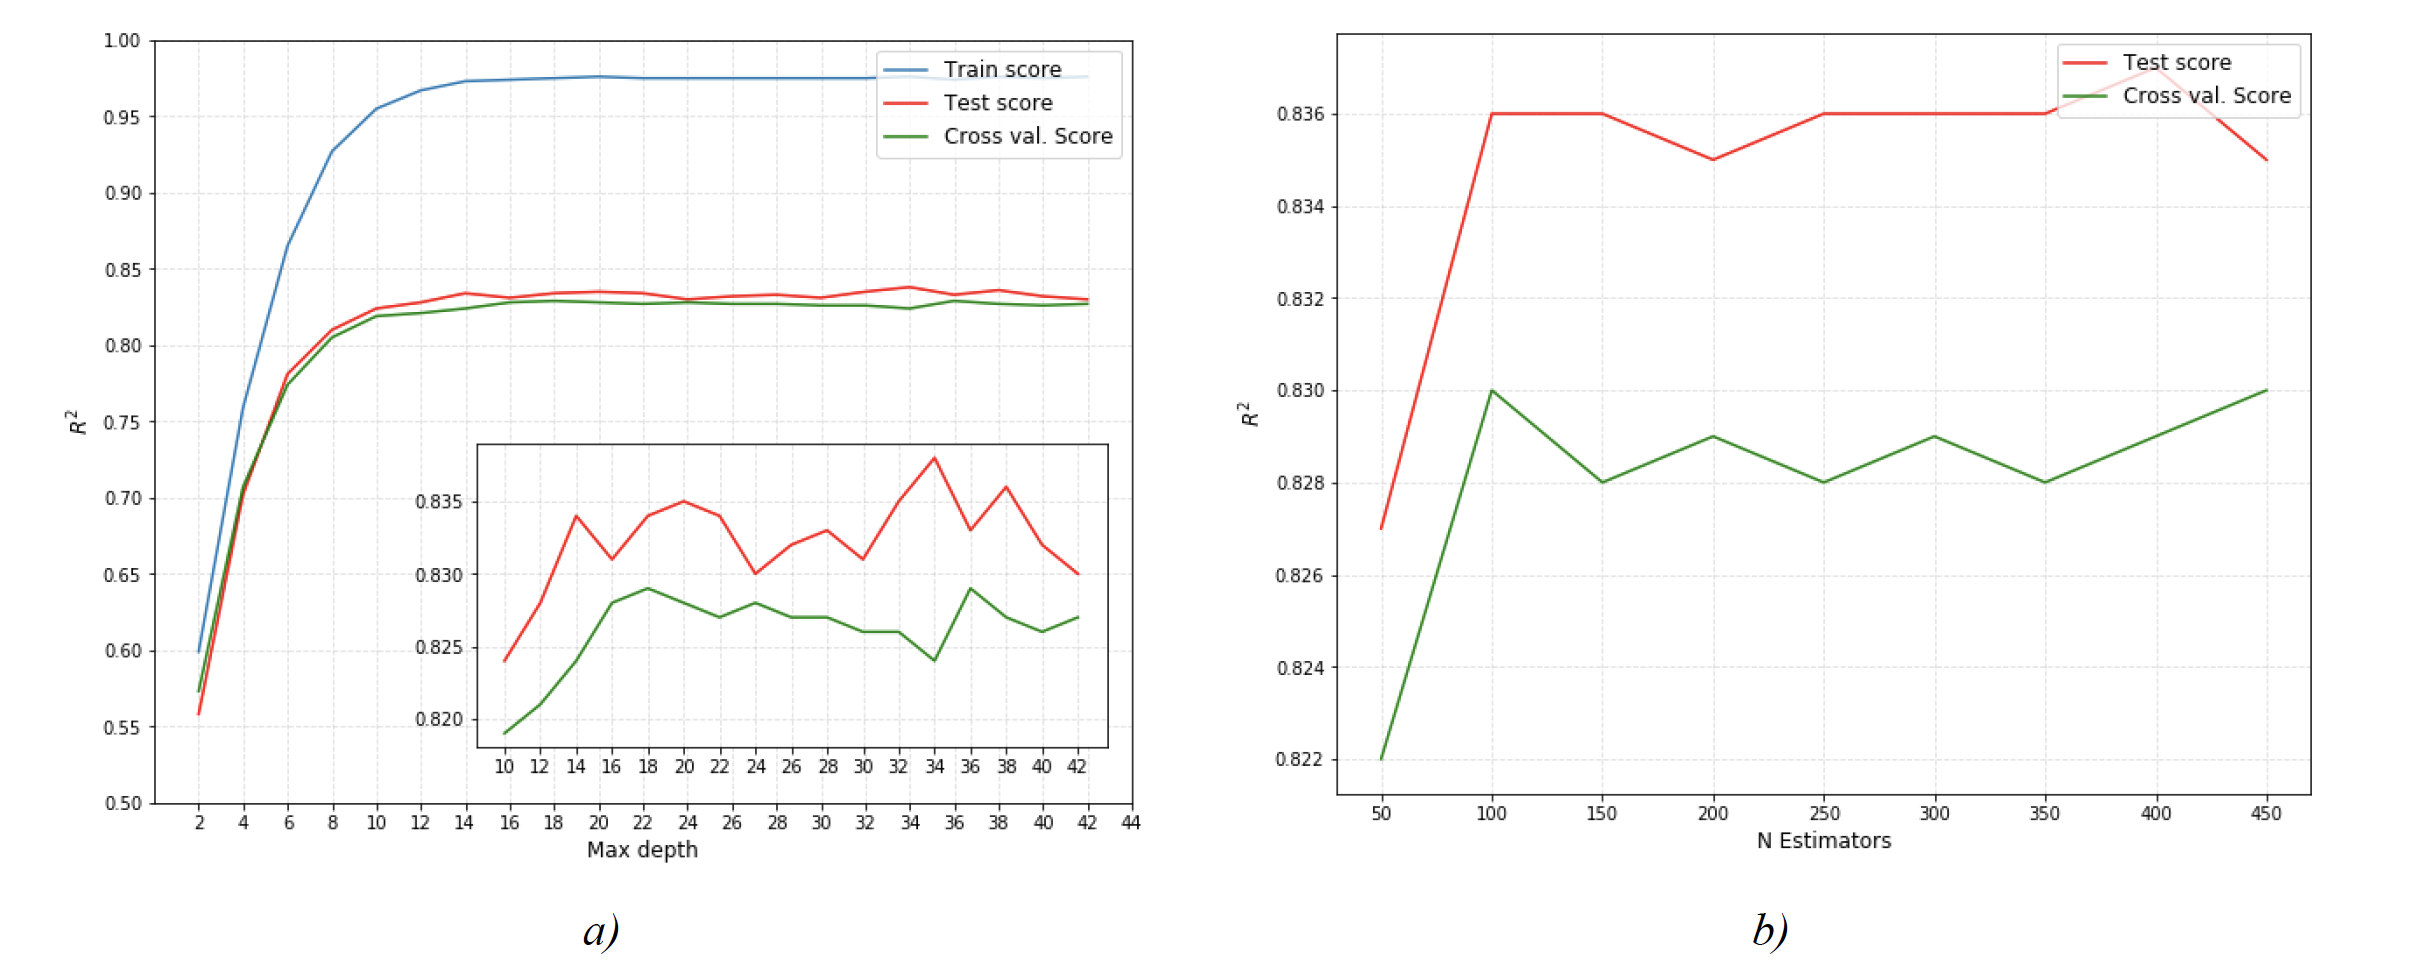
\includegraphics[width=160mm]{fig/ml_fig/rf_convergence.png}
	\caption[RF model hyper parameters tuning.]{RF model hyper parameters tuning a) Convergence with respect to the tree depth b) Convergence with respect to the number of trees.}
\label{fig:rf_convergence}
\end{figure}


\begin{figure}[H]
\centering
\captionsetup{justification=centering,margin=2cm}
	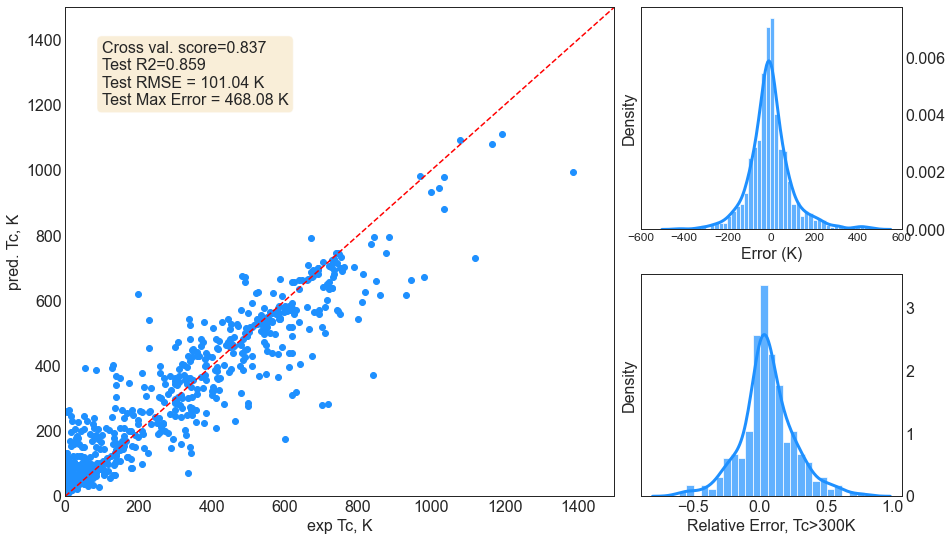
\includegraphics[width=160mm]{fig/ml_fig/rf_results.png}
	\caption[Optimized RF model performance, left comparison of predicted and experimental data.]{Optimized RF model performance, left comparison of predicted and experimental data, right errors and relative errors for the compounds with $T_C>300K$.}
\label{fig:rf_results}
\end{figure}


\begin{table}[H]
\centering
\caption{RF models performance with respect to the features space}
\begin{tabular}{|p{3.5cm}|p{3cm}|p{3cm}|p{3cm}|}
\hline 
Metrics & All & Q75 & Q50 \\ 
\hline 
$R^2$ (test) & 0.833 & 0.819 & 0.810 \\ 
$R^2$ (cross.val) & 0.828 & 0.816 & 0.807 \\ 
RMSE (K) & 109.4 & 113.6 & 131.3 \\ 
Max Error (K) & 516.3 & 540.5 & 601.3 \\ 
\hline 
\end{tabular} 
\label{tab:rf_results}
\end{table}

As it might be seen from the table \ref{tab:rf_results} in general RF outperform the best KRR model and shows good predictive power. Error distribution (Figure \ref{fig:rf_results} right top) shows the relation between experimental and predicted values of critical temperature $(T_C^{exp} - T_C^{pred})$. In our case It is highly symmetrical around zero and might be considered as Gaussian type. From this fact we can conclude that RF model has no systematic bias towards overestimation or underestimation. The distribution of relative errors $(T_C^{exp} - T_C^{pred}) / T_C^{exp}$ showed only for the compounds with $T_C>300K$ since for the compounds with low TC relatively small absolute error may lead to a huge relative one (i.e. for $T_C^{exp} = 1 K$ ; $T_C^{pred} = 15 K$, 1400\% error). Relative error distribution already not so symmetrical but it might be explained due to the low number (136) of samples in it.

\subsubsection{XGBoost alghoritm}
\label{section: XGBoost}

XGBoost is another ensemble algorithm based on decision trees, which utilizes a gradient boosting (GB) framework. Initially, it was designed for small-to-medium structured or tabular datasets, which is exactly the case in this work.
Gradient boosting (GB) is an ML technique very similar to RF.
It produces the prediction model as an ensemble of weak prediction models. The algorithm starts with a single leaf which represents an initial guess for the target variable $(y)$ for the samples, if it is not specified explicitly initial guess is always the average value of $(y)$. The general difference from the simple RF algorithm that GB builds a new tree, based on the errors made by the previous regressor and combines it with the results of the original leaf to make a new prediction. Trees depth in this algorithm controlled by the number of leaves (for regression problems and relatively small datasets <5000 the empirical value of leaves between 8 and 20).
To scale the contribution of each predictor GB use a special parameter called learning rate which is the value between 0 and 1. This parameter is a coefficient that shows the contribution (in RF we couldn’t affect it) of each individual tree to the overall result and also controls the total amount of estimators. Empirical evidence shows that taking lots of small steps in the right direction (use small learning rate) results in a better prediction with testing dataset i.e. lower the variance but also require additional resources. In this work learning rate was set to 0.1 to keep the balance between accuracy and a reasonable amount of computational time.
XGBoost parameter tuning was done according to the general recommended approach:
\begin{enumerate}
\item Firstly, at fixed learning rate was estimated the optimal number of trees as it is shown in Figure \ref{fig:xgb_convergence} (a).
\item Secondly was tuned tree-specific parameters in our case only trees depth see Figure \ref{fig:xgb_convergence} (b)
\item Were determined optimal regularization parameters ($\gamma$, $
\alpha$). These values were set to 1 and 0.5 respectively.
\item Optimization of the learning rate
\end{enumerate}

Therefore, final hyperparameters were as follows: Max depth=8, Number of trees=250, learning rate=0.1, $\gamma=1$,
$\alpha=0.5$.

\begin{figure}[H]
\centering
\captionsetup{justification=centering,margin=2cm}
	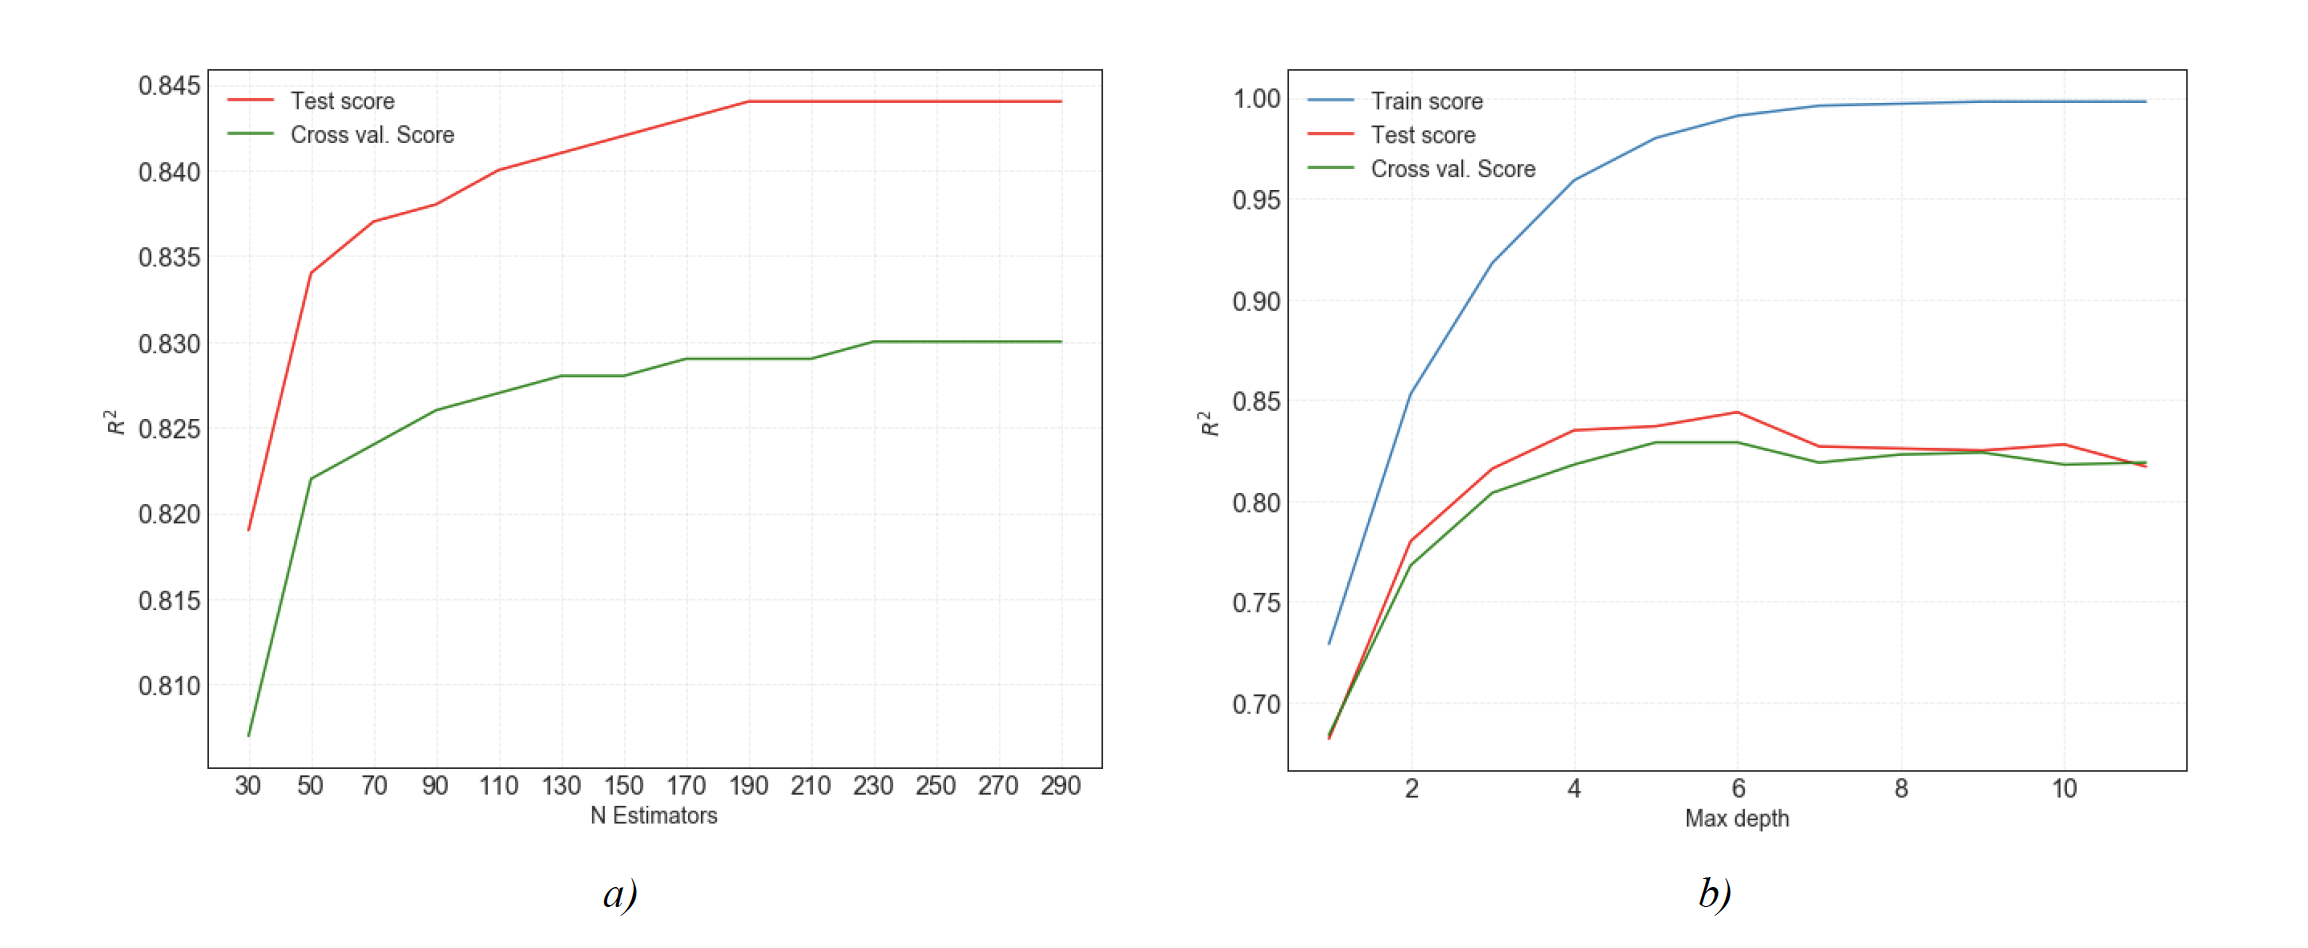
\includegraphics[width=160mm]{fig/ml_fig/xgb_convergence.png}
	\caption[XGBoost model hyperparameters tuning.]{XGBoost model hyperparameters tuning: a) Convergence with respect to the number of trees b) Convergence with respect to the tress depth.}
\label{fig:xgb_convergence}
\end{figure}


\begin{figure}[H]
\centering
\captionsetup{justification=centering,margin=2cm}
	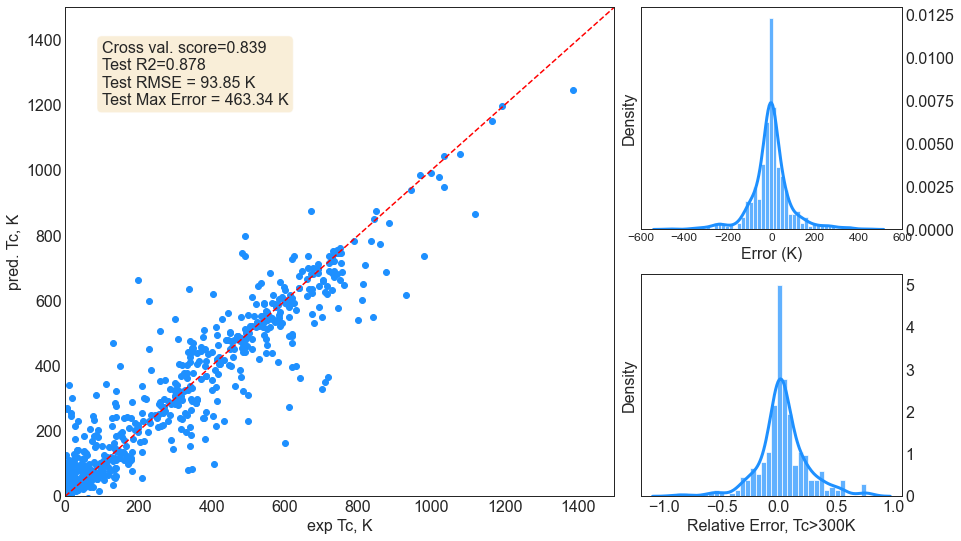
\includegraphics[width=160mm]{fig/ml_fig/xgb_results.png}
	\caption[Optimized XGBoost performance]{Optimized XGBoost performance, left comparison of predicted and experimental data, right errors and relative errors for the compounds with $T_C>300K$.}
\label{fig:xgb_results}
\end{figure}

\begin{table}[H]
\centering
\caption{XGBoost performance with respect to the features space}
\begin{tabular}{|p{3.5cm}|p{3cm}|p{3cm}|p{3cm}|}
\hline 
Metrics & All & Q75 & Q50 \\ 
\hline 
$R^2$ (test) & 0.845 & 0.833 & 0.823 \\ 
$R^2$ (cross.val) & 0.837 & 0.825 & 0.817 \\ 
RMSE (K) & 105.6 & 111.8 & 123.6 \\ 
Max Error (K) & 595.6 & 623.5 & 677.3 \\ 
\hline 
\end{tabular} 
\label{tab:xgb_results}
\end{table}

From the Table \ref{tab:xgb_results} we can conclude that XGBoost in general shows higher accuracy than the RF and KRR. Errors distribution (Figure \ref{fig:xgb_results} top right) is a Gaussian type and highly symmetrical around zero, so this model also has no biases towards the overestimation or underestimation of the $T_C$.

Surprisingly maximum error of this model is sufficiently larger than that one estimated from RF.
Finally, we can conclude that XGBoost is the most accurate model out of all considered in this work with respect to the $R^2$ and $RMSE$ optimization parameters. The mean absolute error $(MAE)$ for this model is 69K.

\subsubsection{Sure independence screening and sparsifying operator (SISSO)}

The sure independence screening and sparsifying operator (SISSO) is a systematic approach for discovering descriptors for materials’ properties, within the framework of compressed-sensing-based dimensionality reduction.
It gives an ability to handle huge and correlated features spaces and converges to the optimal solution building a combination of features relevant to the materials' target property. There are several works \cite{Ouyang_2018,  Ouyang_2019, Ghiringhelli_2015} which report the ability of this algorithm to work efficiently both with regression and classification problems and also to achieve a stable results with relatively small training sets. The output of SISSO is a mathematical model, in the form of explicit, analytic functions of the input physical quantities. This aspect makes this model highly interpretable and gives an opportunity to inspect the equations and obtain some useful physical insights about the problem under consideration.
An input 20-dimensional features space for SISSO were build-out of the 60 most important descriptors which were determined from RF. Were tested different combinations of these features in order to minimize the overall correlation between them. Finally, was constructed a 20-dimensional feature space as it is shown in the correlation matrix (Figure \ref{fig:corr_matrix}).


\begin{figure}[H]
\centering
\captionsetup{justification=centering,margin=2cm}
	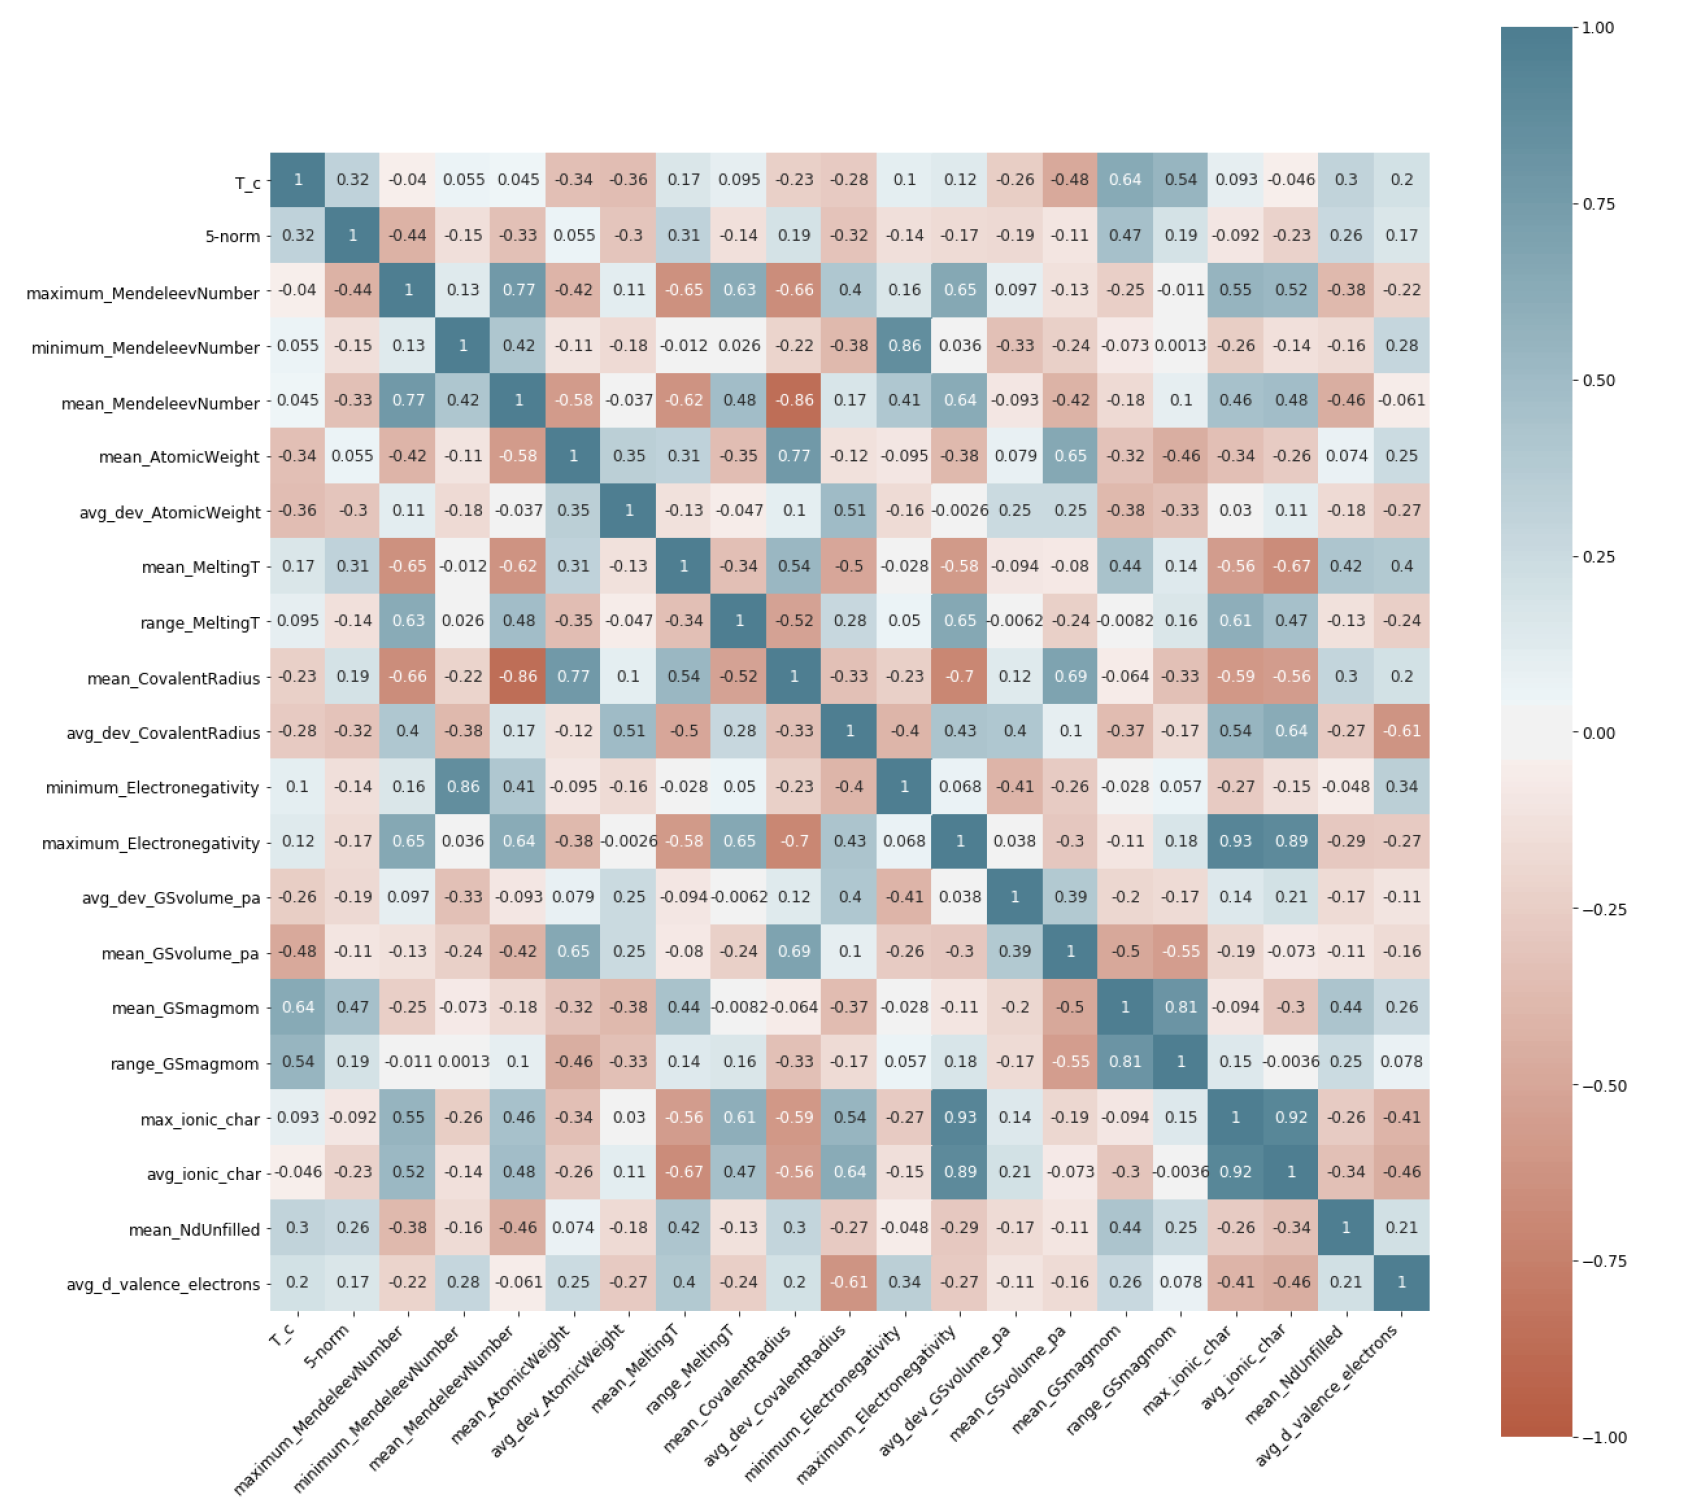
\includegraphics[width=160mm]{fig/ml_fig/corr_matrix.png}
	\caption[Correlation matrix for the most valuable descriptors in RF. ]{Correlation matrix for the most valuable descriptors in RF. These descriptors were used as input for the SISSO algorithm.}
\label{fig:corr_matrix}
\end{figure}

After that SISSO was trained on the entire dataset. Initially, for a baseline model, feature space rung parameter were set to 2, and calculations were performed up to the 7-dimensional descriptor (see Figure \ref{fig:sisso_results}a). As it was expected RMSE and maximum error has a tendency to decrease with the increased size of produced descriptors (see Figure \ref{fig:sisso_results}c).
Then for the second run rung on feature space were increased by one and calculations were also started up to the 7-dimensional descriptor. Unfortunately, only a 3-dimensional (see Figure \ref{fig:sisso_results}b) descriptor was calculated.

\begin{figure}[H]
\centering
\captionsetup{justification=centering,margin=2cm}
	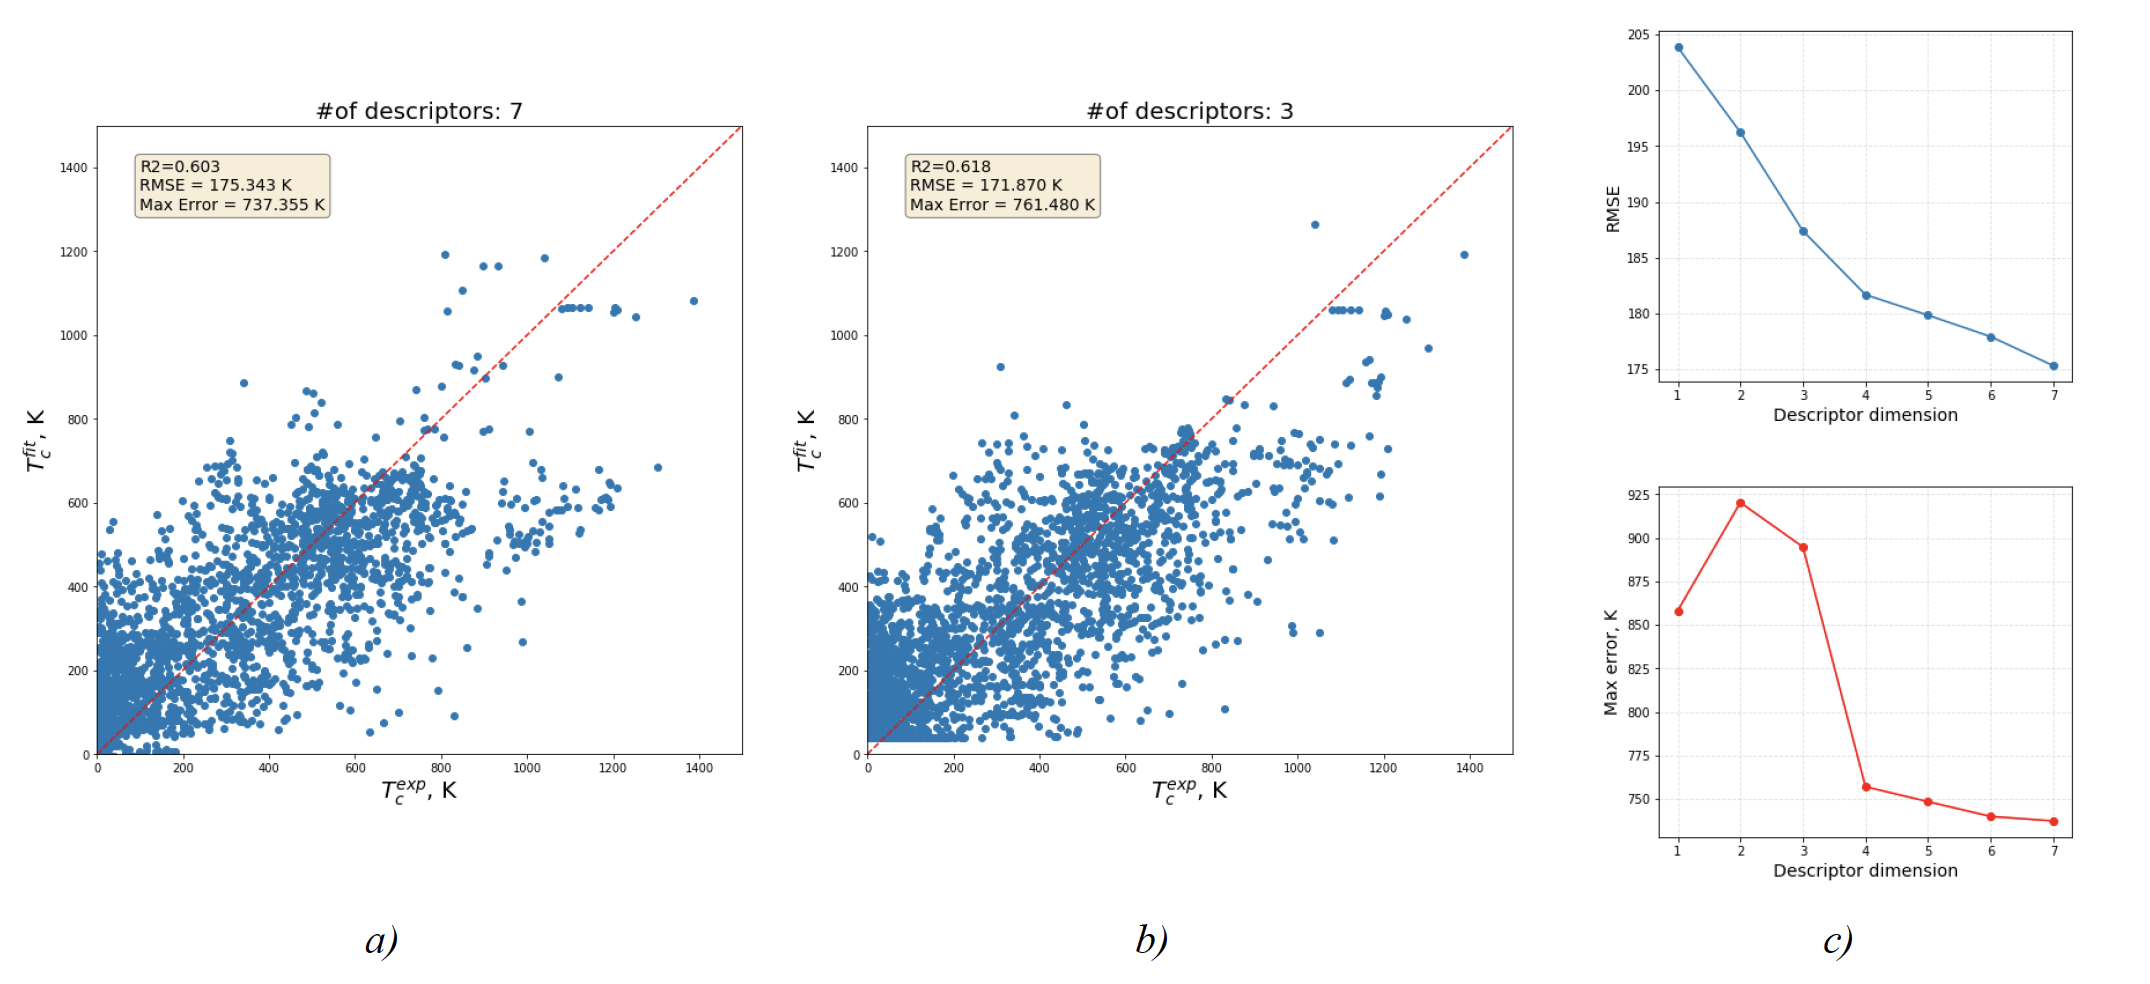
\includegraphics[width=160mm]{fig/ml_fig/sisso_results.png}
	\caption[SISSO model performance.]{SISSO model performance: a) Rung of feature space=3, subspace size=100, b) Rung of feature space=2, subspace size=10, c) RMSE and Max error metrics with respect to the descriptors dimensionality for the feature space with rung 2.}
\label{fig:sisso_results}
\end{figure}

As it is shown $R^2$ value and $RMSE$ metrics for SISSO worse than for the other algorithms. But probably the potential of SISSO is still not fully disclosed and it is possible to achieve a way better result. The only problem is that this algorithm is rather computationally demanding and requires a lot more resources than its available now for the author of this work.
Also, it is interesting to check which features were produced. Here is shown 3 features which were generated during the second run (rung of features space equal to 3):

\begin{align}
& X_1 = \frac{\overline \mu \cdot \varepsilon_{max} \cdot MN_{max}}{\overline V^2 \cdot \overline{T_M} \cdot \Delta T_M}\\
& X_2 = \frac{\overline{N^d} \cdot MN_{min}}{\exp \left( \Delta \mu \right)} - \frac{\overline{N^d} \cdot \overline{MN}}{\exp \left(\varepsilon_{min} \right)}\\
&X_3 = \frac{\left( N^V-\overline{N^d} \right)^2 \overline{\mu} ^ 2}{\varepsilon_{min}^3}
\end{align}


As it might be seen the most frequently used primary features is a magnetic moment $(\overline \mu, \Delta \mu)$ and electronegativity $(\varepsilon_{min}, \varepsilon_{max})$, these features were included in all tree generated descriptors. Features related to the electronic structure namely number of valence electrons $N^V$ and number of electrons on d-shell $(\overline{N^d})$ as well as Mendeleev number $(MN_{min},MN_{max},\overline{MN})$, were included in 2 out of three descriptors. Properties like melting temperature $(\overline{T^M}, \Delta T^M)$ and lattice volume $(\overline{V})$ were used only for one descriptor.

\subsection{Physical understanding of the most important descriptors}

Building an efficient model that could make an accurate prediction is an important part of the ML pipeline. But what is even more important is to interpret your model properly and find what kind of physical insights and understanding of a particular problem might be extracted from it. That's why in some cases simpler models like decision trees or Random Forest are more preferable due to their high interpretability and transparency.
Figure \ref{fig:rf_features} shows the histogram of the top 15 most valuable features which were extracted from our trained RF model. Actually, this feature is not strongly different between 3 of our models (KRR, RF and XGBoost), that's why it's enough to consider only one such histogram.

\begin{figure}[H]
	\centering
	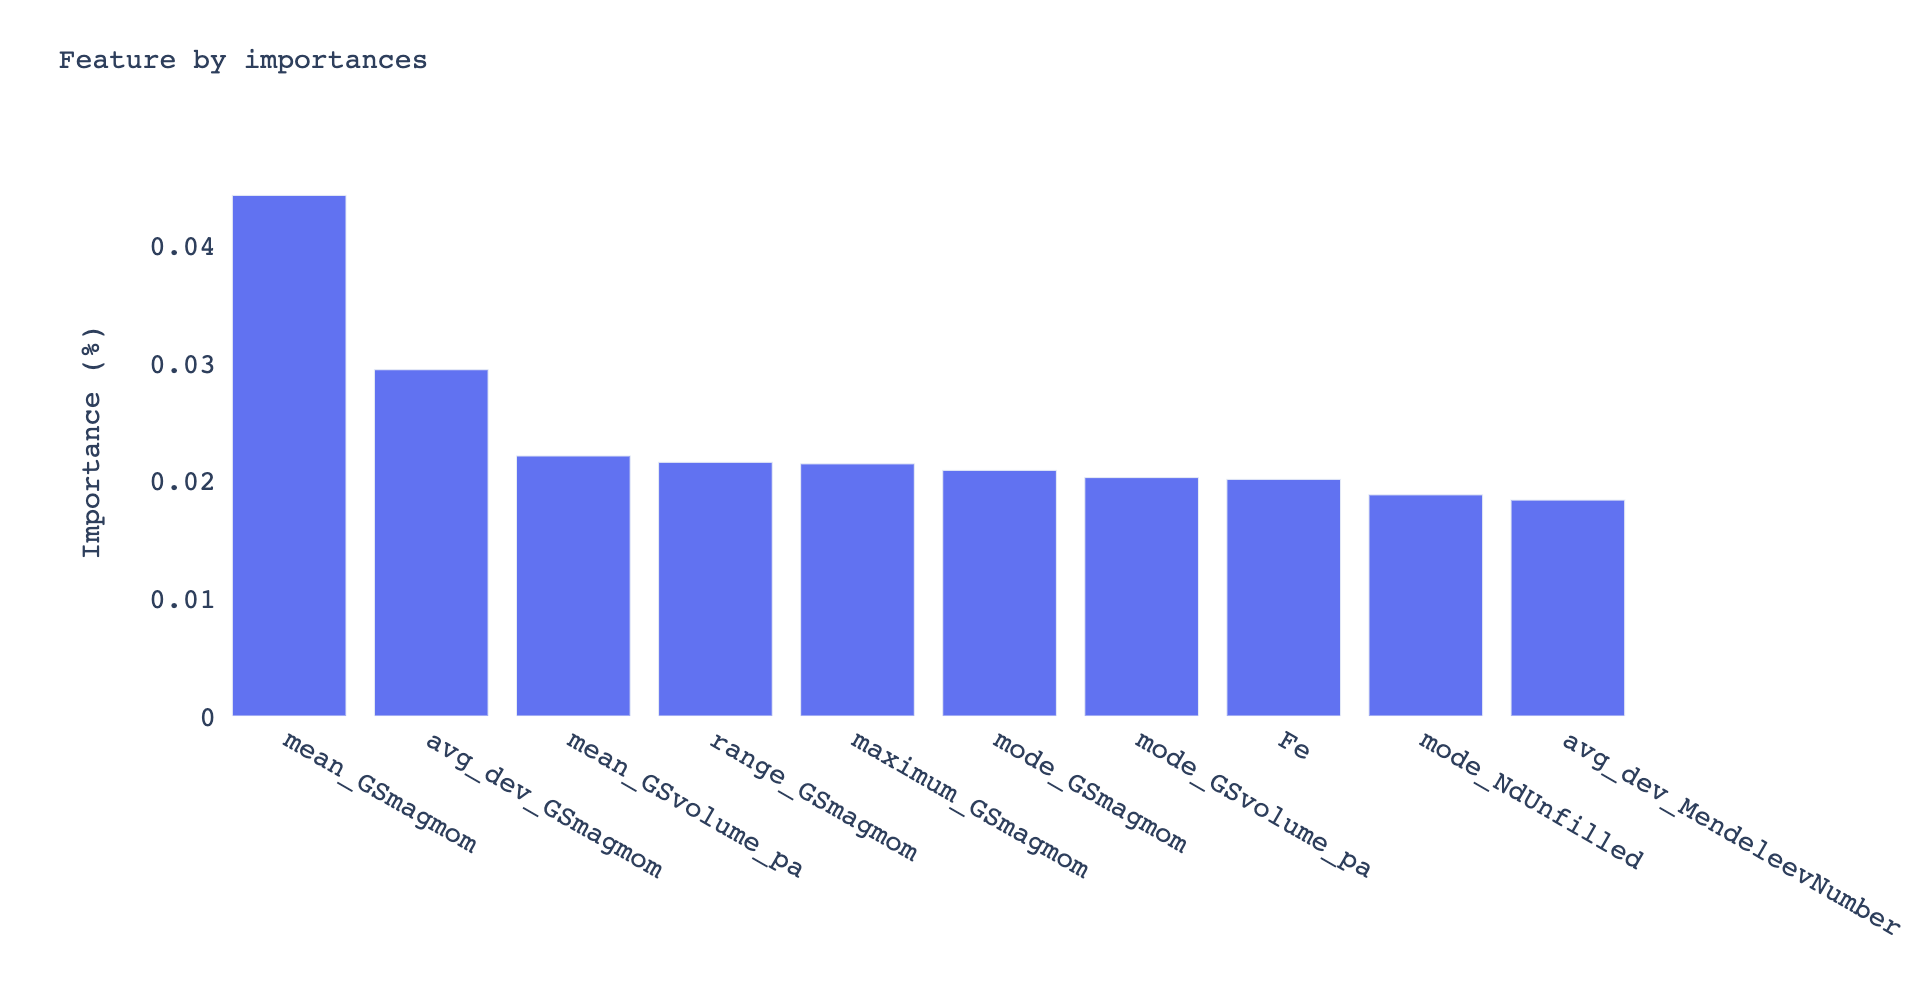
\includegraphics[width=140mm]{fig/ml_fig/rf_features.png}
	\caption[RF feature importance histogram.]{RF feature importance histogram.}
\label{fig:rf_features}
\end{figure}

Five descriptors out of fifteen related to the magnetic moment, namely: $\mu_{max}, \Delta \mu,  \overline{\mu}, \tilde{\mu}, \langle \mu \rangle$. This fact is quite understandable since by definition target property $(T_C)$ is a point of sharp changes in the magnetic properties.
There are 2 descriptors corresponding to the atomic fraction of particular elements, namely Iron (Fe) and Cobalt (Co) it is also might be explained due to their strong ferromagnetic nature, other important elements like Nickel (Ni) and Manganese (Mn) are 25th and 40th respectively.
There 2 features related to the number of electrons on d-shell $\overline{N^d}, \widetilde{N^d}$ and again it’s a well-known fact that partially filled d-shell usually correlated with nonzero total spin and thus magnetism.
Also, there 2 descriptors related to lattice volume $\overline{V}, \widetilde{V}$, this already not so trivial, but probably related to the phenomena of the exchange coupling which is strongly dependent on the number of nearest neighbours in the crystal structure.
Comparing the most valuable features extracted from KRR, RF, and XGBoost with the features computed from SISSO we may say that they have a lot in common despite the fact that all these algorithms use different mathematical approaches and approximations.




\cleardoublepage
\section{DFT + MC calculations of critical temperature}

\label{section: DFT_MC}

One of the foundation stones of this particular work is developing a stable and efficient method for estimating ferromagnetics critical temperature (Curie temperature). In a framework of described in section \ref{section: Magnetic models} spin model, it is straightforward that the main parameter which should be found to conduct this calculation is exchanged interaction $J_{ij}$. Finding this parameter allows to carry out Monte Carlo simulation as it is described in section \ref{section: Monte Carlo method}  for the precise description of the system's thermodynamic properties or apply less computational demanding but yet quite accurate Curie-Weiss approximation.  Steps required for these purposes are schematically illustrated in figure \ref{fig:End-to-end pipeline scheme} and described in more detail in upcoming sections.


\subsection{Obtain initial geometry}
On a stage of development and validation of algorithm, this work used FM structures with known magnetic properties, and critical temperature preferably obtained both from experimental and theoretical studies. In particular was used structural information provided by the Materials Project and NOVOMAG databases, which have already proven as a reliable tool for computational materials exploring. 

\subsection{Generation of spin configurations}
From obtained structural information of a parent FM cell, one may generate various derivative structures with specified AFM properties (i.e., ratio of spin-up and spin-down atoms is 1:1) utilizing existing algorithms for derivative structure generation. 
For these purposes, currently used open-source python library, \textit{pymatgen} \cite{Ong:2013vd} with integrated derivative structure generator \textit{enumlib} \cite{enum_1, enum_2, enum_3, enum_4}. Based on symmetry analysis its generates different AFM spin configurations from the parental FM. One of the big advantages of the current derivative structure enumerator is the possibility of eliminating the heuristics-based approach. On the contrary of producing a huge number of randomly oriented spin configurations with the hope of getting the one that is close enough to FM ground state, it makes a rigorous and thus reliable search for all possible spin states. The number of obtained spin configurations we may consider almost exhaustive, which is also proven in a series of studies by comparing with experimental data. \cite{Zhu_2018, Jiang_2018} .

\subsection{Energy calculations}

Initial FM cell, as well as various generated AFM structures, are then relaxed using collinear density functional theory,  and their energies are accurately calculated.  

Spin-polarized DFT calculations are carried out using generalized gradient approximation (GGA) as implemented in the Vienna Ab initio Simulation Package (VASP) \cite{Kresse_1996} with projector augmented-wave (PAW) \cite{Kresse_1999} method applying the Perdew–Burke–Ernzenhof (PBE) \cite{Perdew_1996} exchange-correlation functional. For all calculations was used sufficiently large value of cut-off energy up to 1.5 of the maximum provided in pseudopotential file.

Because the energy differences between various close to ground state spin configurations are usually on several milli-electron volts (meV), it's essential to conduct computations with sufficiently high accuracy but also keep computational demanding on a reasonable limit. To keep the balance between efficient usage of computational resources and accuracy requirements, stages of relaxation and static energy calculations use a step-by-step approach (with increasing accuracy). This way allows to quickly determine unsuitable for the future calculations structures and exclude them saving resources.

For the relaxation stage was employed gamma-centered grid with the default specified in VASP reciprocal density of 64 \AA $^{−3}$ while the static calculations utilize significantly higher reciprocal density of 300 \AA $^{−3}$ . This type of mesh is known to be a pretty flexible (and probably the most commonly used) flavor of the automatic grid generation mode and is shown to achieve faster energy convergence compared to standard Monkhorst-Pack grids.

The parameter of electronic convergence (energy difference between successive electronic steps) is varying from $10^{-4}$ eV for the initial relaxation stages up to  $10^{-6}$ eV for the finalizing static runs.

Worth mentioning that at this step, it is essential to ensure that among all produced spin configurations, the ground state is found to be FM. Otherwise (AFM structure is ground state), it is needed to treat this material differently, and the workflow cannot be continued.  Another important step is to check if all the structures kept their local magnetization unchanged (or at least these changes are not significant). Quite often, especially structures with low initial magnetic moments exhibit total disappearance of magnetization in AFM state. Such behavior makes them absolutely nonmagnetic and thus not representative for further Hamiltonian fitting.

For the case of structures with strongly correlated d-shell electrons, it was also tested Hubbard correction approach (GGA + U) using the Dudarev \cite{Dudarev_1998} formulation which is proven to give accurate results for such systems.  

The effective U values for transition metals calibrated by performing a fitting to experimental binary formation enthalpies have been taken from the Materials Project website \cite{Wang_2006}.
This is a common practice and has already shown reasonable results in a high-throughput screening study performed in ref. \cite{Zhu_2018}. 
Of course, usage of Huburd correction values without proper calibration, for instance, by linear response method \cite{Cococcioni_2005},  may lead to unsatisfying results, especially for structures containing elements with relatively low magnetization. Unfortunately, the computational demand of such calibration is sufficiently large and not applicable in high-throughput calculations.


\subsection{Hamiltonian fitting}

\subsubsection{Building the system}
The energies calculated at the previous stage for the relaxed parental FM and derivative AFM configurations make it possible to determine the exchange coupling parameters $(J_{ij})$. For these purposes initially carried out mapping of magnetic neighbors in every generated spin configuration utilizing \textit{pymatgen} \cite{Ong:2013vd} and \textit{siman} \cite{Aksyonov_2018} libraries . This stage performed not only mapping of magnetic nearest (mNN) and next-nearest magnetic neighbors (mNNN), located in the first and second coordination spheres respectively, the search is extended to the higher-order coordination spheres up to the number of generated spin configurations.
Hence for any FM system with a number of generated AFM spin configurations equal to $N$, mapping was done up to the $N-th$ coordination sphere in every structure (e.g., for 6 generated AFM structures, mapping of magnetic neighbors performed up to the 6-th coordination spheres).

Mapping procedure returns a series of coefficients $(n_{ij})$ which, with the addition of calculated energies $(E_{FM/AFM})$ , allows building a system of equations. Produced system includes $N + 1$ equations ($1$ FM + $N$ AFM configurations) and $N + 1$ variables $(E_g, J_1, ... J_n)$. 

\begin{equation}
  \left\{
    \begin{aligned}
      & E_g + n_{11}J_1 + \hdots + n_{1N} J_n = E_{FM}\\
      & E_g + n_{21}J_1 + \hdots + n_{2N} J_n = E_{AFM1}\\
      &\vdots\\
      & E_g + n_{N1} J_1 + \hdots + n_{NN}J_n = E_{AFM_N}
    \end{aligned}
  \right.
\end{equation}


Its might be illustrated on the toy example from figure \ref{fig:spinupdown}. Suppose we have a 2D structure with a spin-up red atoms and spin-down blue atoms.  As a 1st nearest neighbors of our spin-up central atom, we have 4 atoms with an antiparallel spin which means that sign of their interaction will be negative. Building the second coordination sphere we can see that all 2nd neighbors have the same spin with the central one, therefore, the sign of their interaction will be positive. 

\begin{figure}[H]
\centering
\captionsetup{justification=centering,margin=2cm}
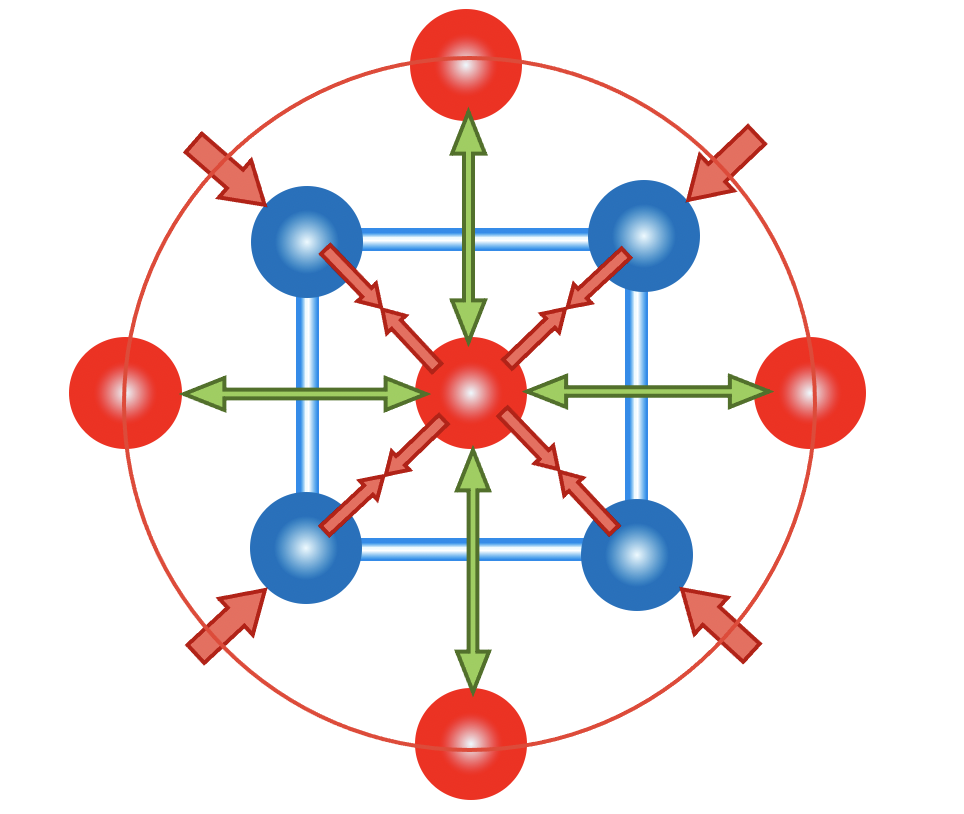
\includegraphics[width=80mm]{fig/dft_fig/spinupdown.png}
\caption{Schematic determination of $J_1$ and $J_2$ coefficients in $2D$ case.}
\label{fig:spinupdown}
\end{figure} 


Hence the total energy of the given ferromagnetic system can be written as:
\begin{equation}
E_{AFM}=E_{g}-4J_1+4J_2
\end{equation}

Where $E_g$ – corresponds for the part of energy given by the geometry itself.


\subsubsection{Solving the system}

Extracting values of exchange couplings from the produced systems were done in two different methodologies.

In the case of a nonzero determinant, it is possible to obtain an exact solution directly solving the system. 

\begin{equation}
\det\begin{pmatrix} 
n_{11} & \hdots & n_{1N} \\ 
\hdots &  & \hdots\\
n_{21} & \hdots &  n_{NN} 
\end{pmatrix} \neq 0
\end{equation}


Otherwise, the less stable (with the highest energy) AFM configuration is excluded from the calculations until the equations system becomes solvable or runs out of the structures. This method has obvious disadvantages. Firstly quite frequently from the mapped coefficients, it's impossible to build any solvable system, and the calculations fail. Secondly, excluding less favorable spin configuration from the solution, one by one, frequently leads to a minimal possible system $2\times2,$ which returns only the $J_1$ parameter and thus makes the results poorly representative for the further $T_C$ estimation.

The second methodology utilizes a common strategy applicable for overdetermined systems, namely the least-squares method. In this study, fitting was done starting from the $N \times N$ system, continually decreasing the number of taken into account variables up to the $N \times 2$ $(E_g, J_1)$. Such an approach allows to better distinguish strong and weak exchange correlations in the materials showing how every group of magnetic atoms located on a particular coordination sphere contribute to the final exchange values. Worth mentioning that contrary to the direct system solving this approach is extremely sensitive to the quality of all the produced AFM structures. In other words,  any poorly relaxed or disordered physically meaningless structure that might appear in the system won't be excluded at any stage and strongly affect all the produced results.
For clarity let's consider a couple of examples, namely FM Mn and Eu oxides.

\subsubsection{Example 1}

For the case of \ce{EuO} were generated 3 unique AFM cells (see figure \ref{fig:example_1}). Based on the energies of given structures obtained from the spin-polarized DFT calculations, one may build a system of 3 equations that has 3 variables $(E_g, J_1, J_2)$. Since the coefficients obtained for a given system form a nonzero determinant, this system can be solved exactly.

\begin{figure}[H]
\centering
\captionsetup{justification=centering,margin=2cm}
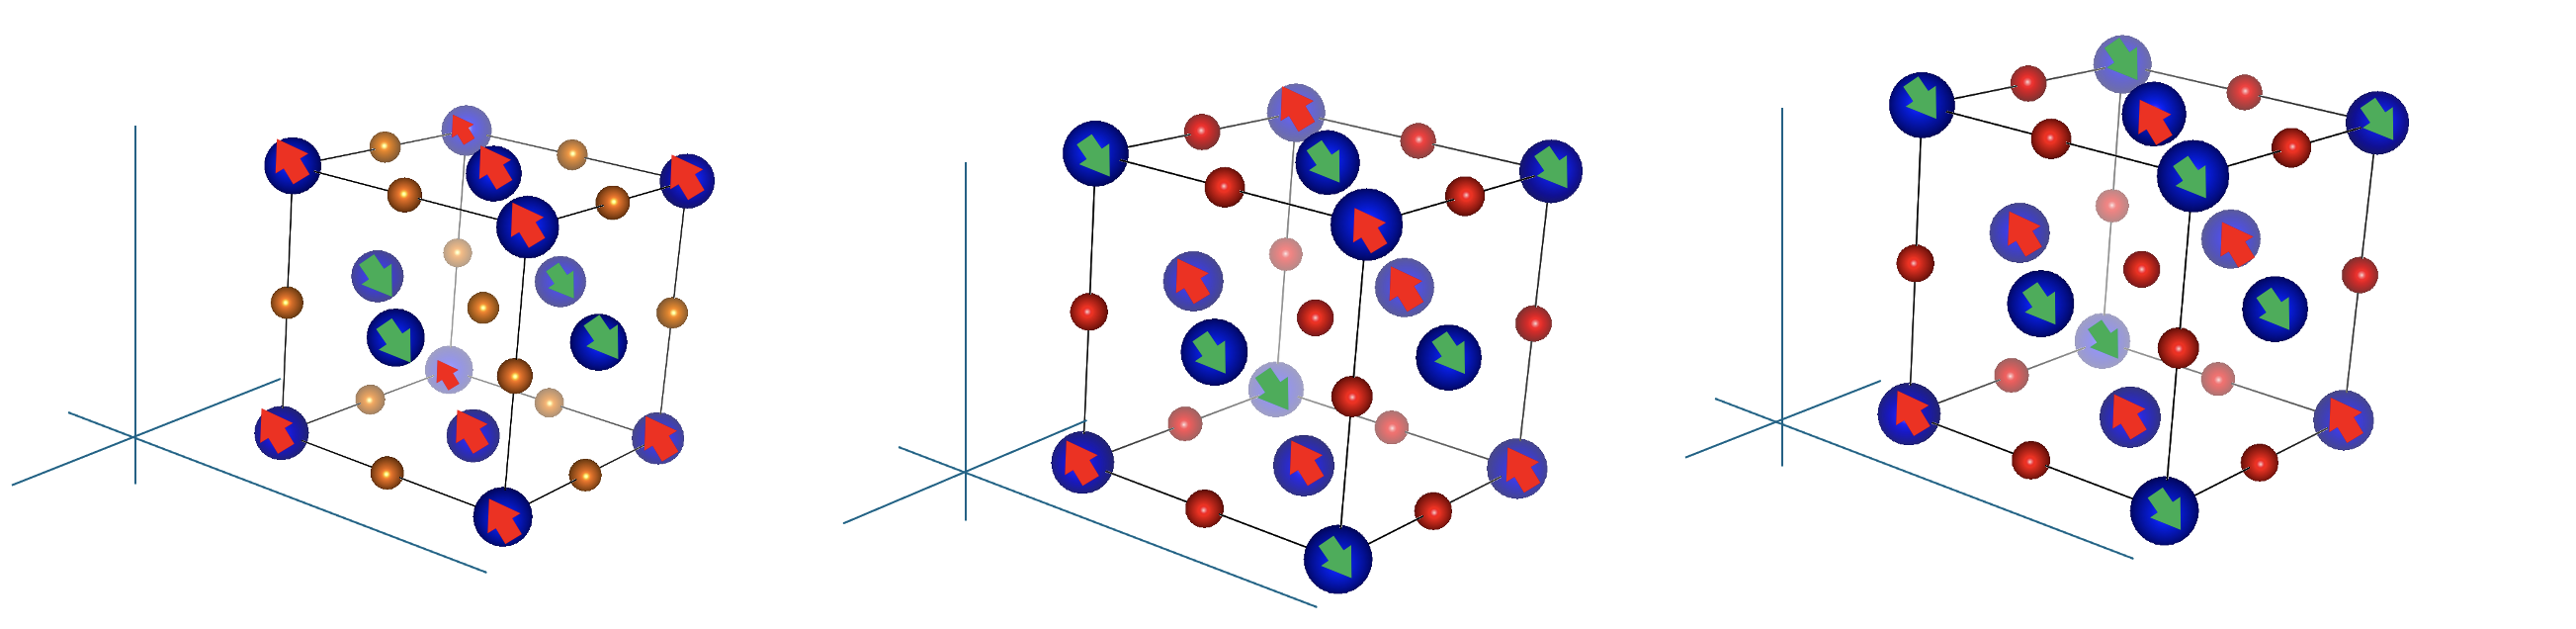
\includegraphics[width=160mm]{fig/dft_fig/example_1.png}
\caption[Three different spin configurations produced for \ce{EuO}.]{Three different spin configurations produced for \ce{EuO} that allows to calculate the $J_1$ and $J_2$ exchange couplings.}
\label{fig:example_1}
\end{figure}

\begin{multicols}{2}
\begin{equation}
  \left\{
    \begin{aligned}
      & E_g + 4J_1 - 6J_2 = E_{AFM1}\\
      & E_g + 0J_1 + 6J_2 = E_{AFM2}\\
      & E_g - 4J_1 - 2J_2 = E_{AFM3}
    \end{aligned}
  \right.
\end{equation}

\begin{equation}
    \begin{aligned}
      & E_{g} =−41.63324\ eV\\
      & J_{1} =1.18\ meV\\
      & J_{2} =0.42\ meV \\
      & T_C^{GGA} = 69\ K \\
      & T_C^{exp.} = 67\ K
    \end{aligned}
\end{equation}
\end{multicols}


Solution of the system allows calculating exchange coupling parameters for the first and second coordination spheres $(J_1, J_2)$.  As it might be seen from the calculated values, in this case, exchange couplings have the order of meV. This fact once again points out the critical importance of extremely accurate relaxation and energy estimation steps. The calculated value of critical temperature $67K$ is in perfect agreement with the experimental value of $69 K$.

\subsubsection{Example 2}

For the case of \ce{MnO} were considered 3 spin configurations (parental FM and two generated AFM). In the same manner, for the given structures were performed accurate relaxation followed by single-point energy calculations. 

\begin{figure}[H]
\centering
\captionsetup{justification=centering,margin=2cm}
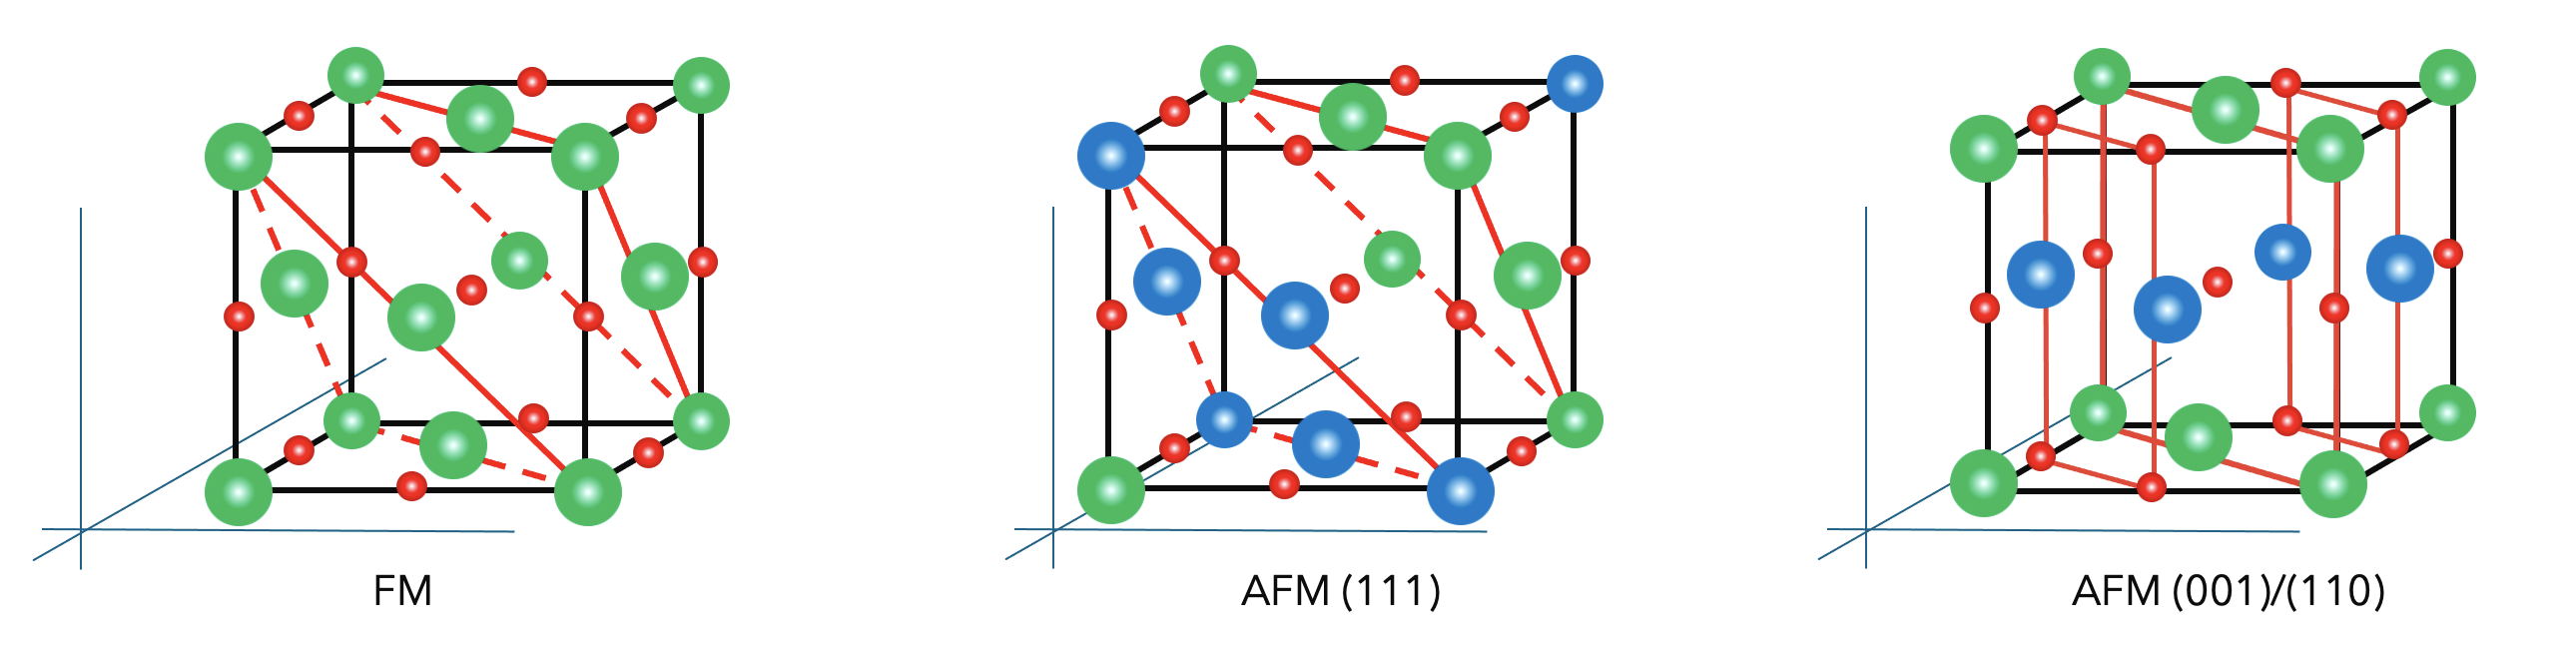
\includegraphics[width=160mm]{fig/dft_fig/example_2.png}
\caption[Three different spin configurations
produced for MnO.]{Three different spin configurations
produced for MnO that allows to calculate the $J_1$ and $J_2$ exchange couplings.}
\label{fig:example_2}
\end{figure}

\begin{multicols}{2}
\begin{equation}
  \left\{
    \begin{aligned}
      & E_g + 6J_1 + 3J_2 = E_{FM}\\
      & E_g - 2J_1 + 3J_2 = E_{AFM1}\\
      & E_g +0J_1 - 3J_2 =  E_{AFM2}
    \end{aligned}
  \right.
\end{equation}

\begin{equation}
    \begin{aligned}
      & J_{1} =9.50\ meV\\
      & J_{2} =14.91\ meV \\
      & T_C^{GGA+U} = 249\ K \\
      & T_C^{exp.} = 118\ K
    \end{aligned}
\end{equation}
\end{multicols}

Obtained values of exchange coupling for the first $(J_1)$ and second coordination spheres $(J_2)$ on the order of several meV. In this case, the estimated value of critical temperature $T^{GGA+U}_C = 249 K$ overestimates the experimental one $T^{exp.}_C = 118 K$ more than two times. Nevertheless, results still might be considered valuable since they allow to distinguish structures with doubtful technological potential.

One more important point here is the quite a noticeable difference between the experimental values obtained for the system under consideration by different groups. For instance $90 K$ in ref. \cite{Lines_1965}, while ref. \cite{Roth_1958} reported $118 K$ and the most recent results of $85 K$ in ref. \cite{Pepy_1974}. This variability also raises how it is correct to compare theoretically estimated values with experimentally obtained. Since samples of the same material might have a different quality and even small defects might strongly affect the magnetic properties. While varying experimental techniques and differ in equipment might lead to even bigger divergence. This fact was also briefly discussed during the description of the data pre-processing  in section \ref{section:Data pre-processing}

\subsection{Monte Carlo simulation} 

As a final step of the workflow values of exchange coupling parameters $(J_{ij})$ used to study the material transition from ferromagnetic (FM) to paramagnetic (PM) state. It is done by the source of constrained Monte Carlo (MC) \cite{Evans_2010} metropolis algorithm as implemented in Vampire \cite{Evans_2014, Evans_2015} software which allows to carry out calculations of the equilibrium temperature-dependent magnetic properties. Vampire contains a predefined functionality to estimate critical temperature by performing a temperature sweep and calculating the average magnetization, returning the classic M-T curve.

For all the systems, exchange energy was considered isotropic (equal in all directions). To neglect finite-size and surface effects in a bulk material was chosen sufficiently large dimensionality of $10 \times 10 \times 10\ nm^3$ and defined periodic boundary conditions in all three spatial directions.  Temperature range of modeling was specified from $0$ to $1500\ K$ with an increment of $25\ K$ for each temperature done $10^5$ equilibration time steps which is needed to reach thermal equilibrium in the system followed by the $10^5$ loop-time steps, which is already counted to the average of magnetization as it is illustrated in figure \ref{fig:time_magnetization}.  Quite a large number of equilibration steps explained due to known equilibration-temperature dependence which tends to drastically slow down close to the Curie point. Specified numbers chosen heuristically but yet yields reasonable results for the most of systems.
The bigger number of averaging steps, in general, lead to more smooth data but obviously requests more computational resources.

\begin{figure}[H]
\centering
\captionsetup{justification=centering,margin=2cm}
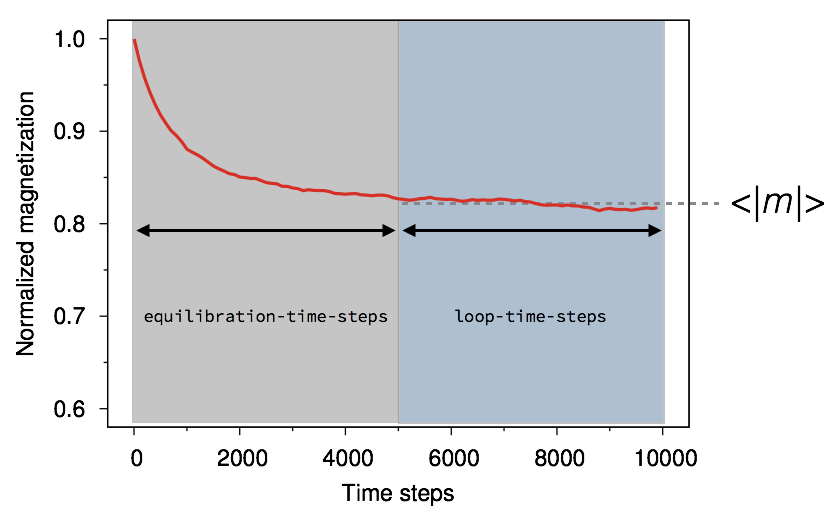
\includegraphics[width=120mm]{fig/dft_fig/time_magnetization.png}
\caption[Time-dependent magnetisation caused by a stepwise increase in temperature.]{Time-dependent magnetisation caused by a stepwise increase in temperature.}
\label{fig:time_magnetization}
\end{figure}

As a result of running MC simulation returns data for the magnetization-temperature curve as it is shown in figure \ref{fig:mt_curve}, from which one may determine the critical temperature as point with a maximum gradient. 

\begin{figure}[H]
\centering
\captionsetup{justification=centering,margin=2cm}
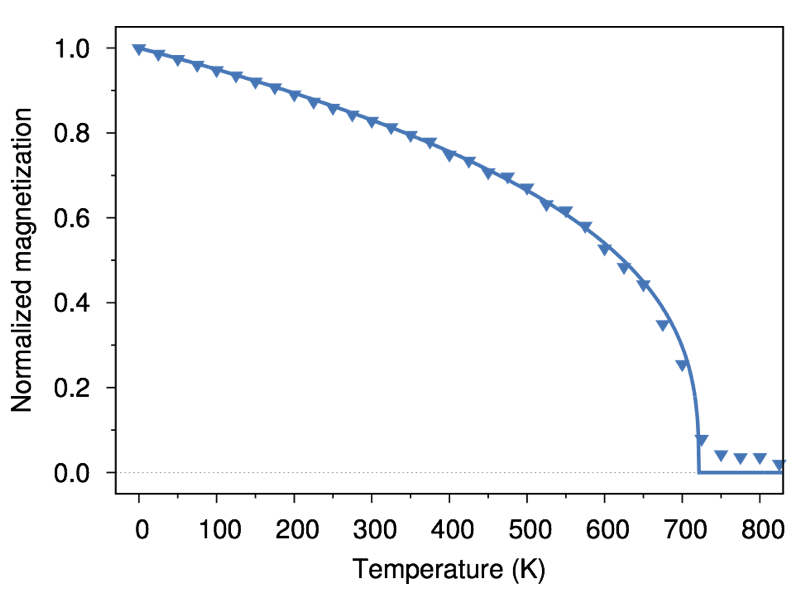
\includegraphics[width=120mm]{fig/dft_fig/mt_curve.png}
\caption[MC magnetization temperature curve.]{MC magnetization temperature curve.}
\label{fig:mt_curve}
\end{figure}

\subsection{End-to-end pipeline details} 
All pieces of the code for integration with side packages and data pre/post-processing produced during the work were formed into a complete end-to-end Python-based package. The main goal of the prepared package was to automate all the stages of the critical temperature calculations, eliminating the need for user control and making it usable for any FM material.  Schematically algorithm shown in figure \ref{fig:End-to-end pipeline scheme}.

\begin{figure}[H]
\centering
\captionsetup{justification=centering,margin=2cm}
	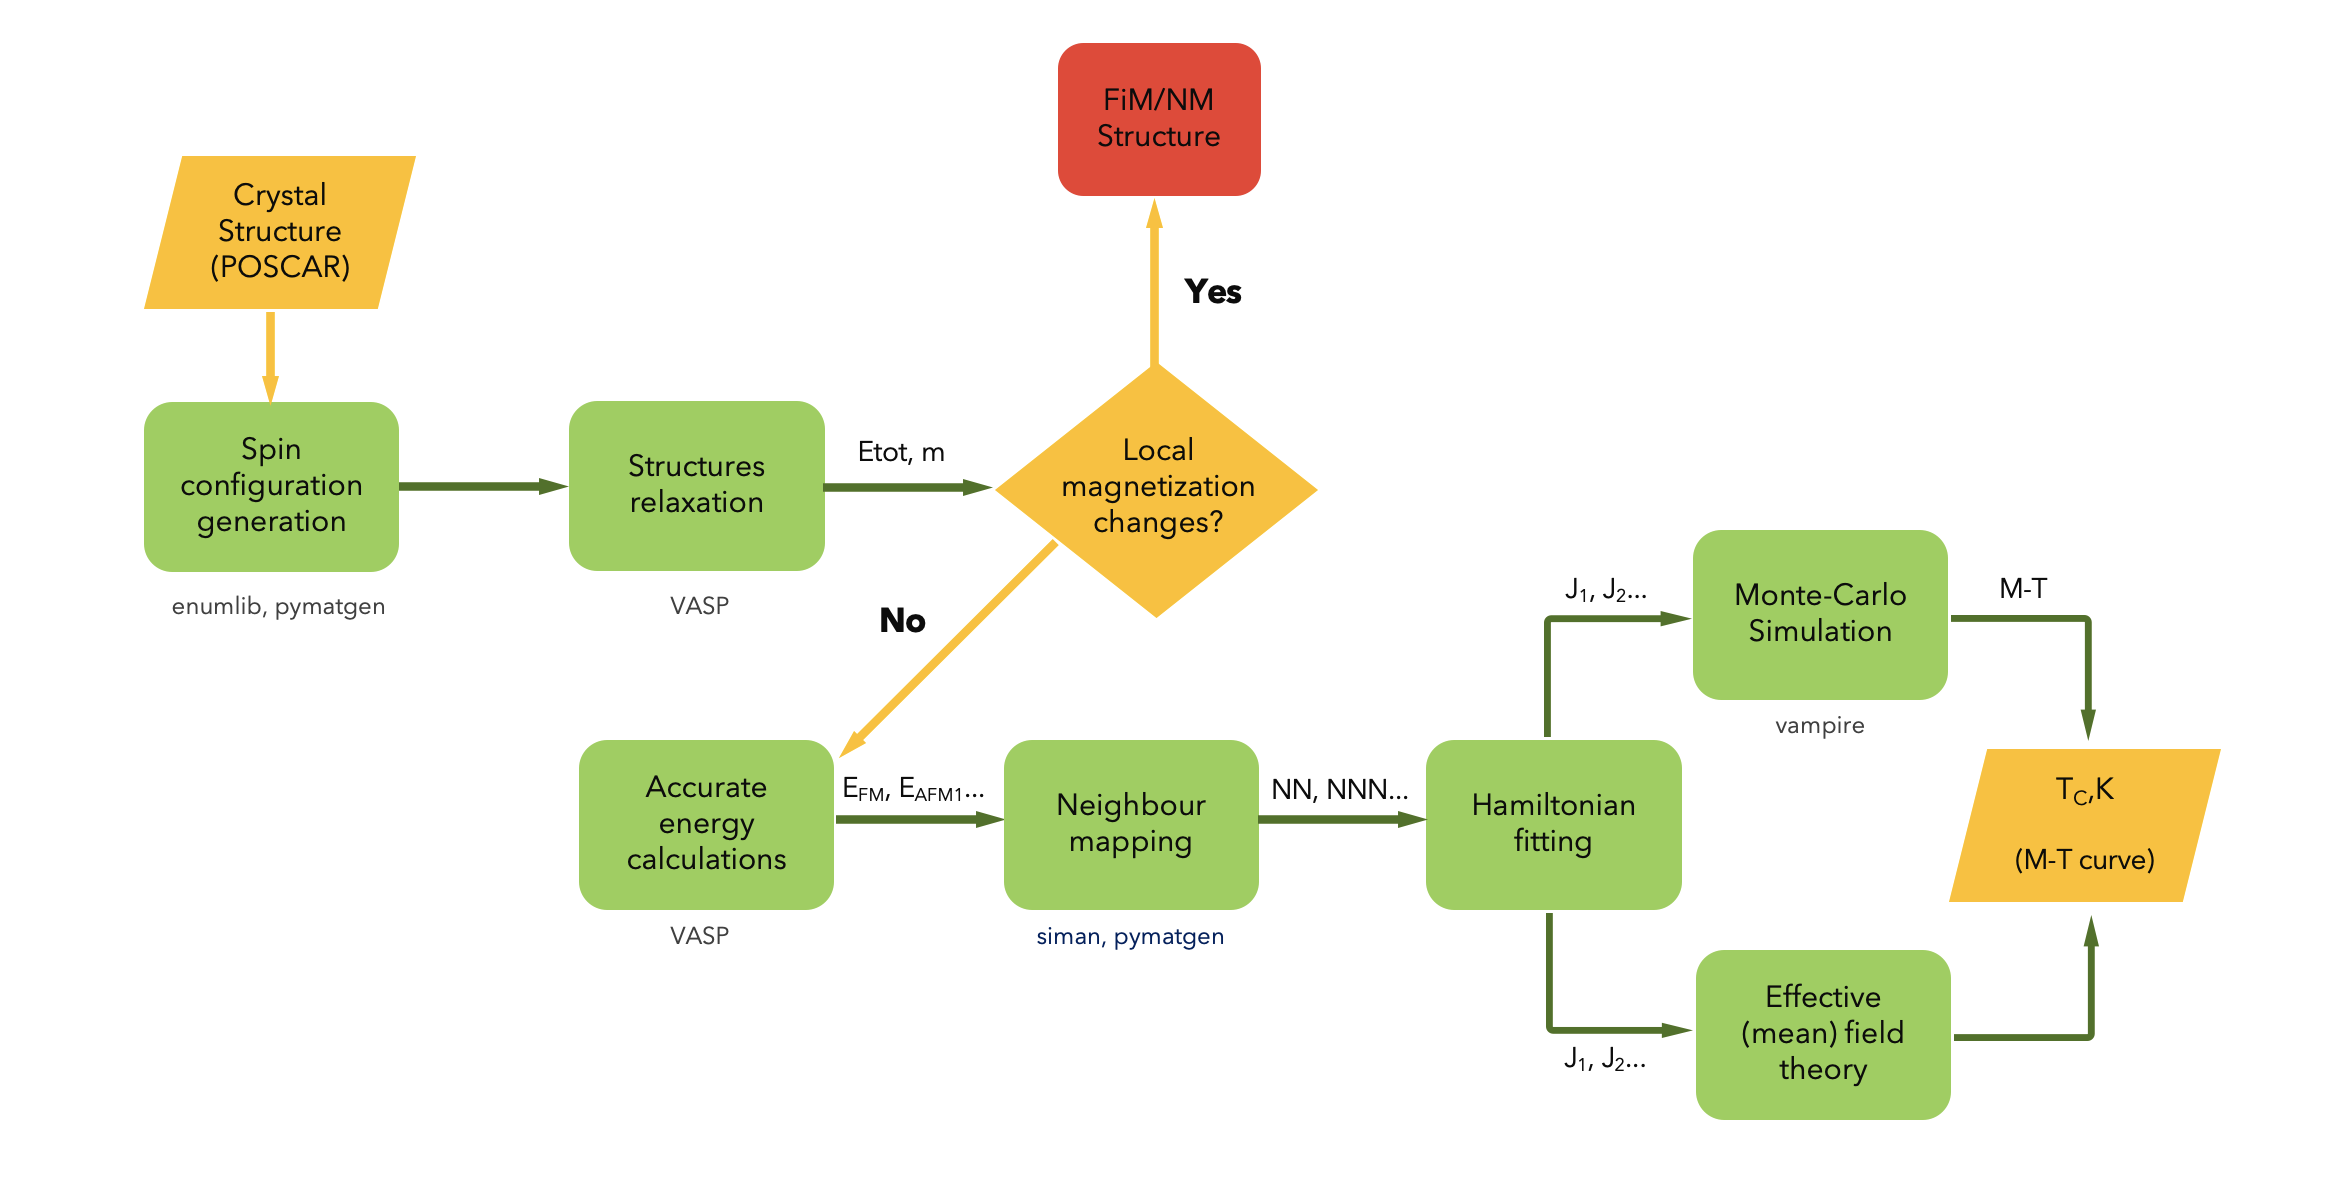
\includegraphics[width=160mm]{fig/dft_fig/algo.png}
	\caption[End-to-end pipeline scheme.]{End-to-end pipeline scheme.}
\label{fig:End-to-end pipeline scheme}
\end{figure}

The package was built with the philosophy to be suitable even for people without special knowledge in electronic structure calculations keeping the entry barrier as low as possible.
In the architecture of the code, we tried to save a balance between being simple for the novice yet maintaining flexibility for advanced users who know exactly what it does. 
As minimum input information its only needs to provide crystal structure data in a form of a commonly used POSCAR type file. All the required parameters for calculations by the DFT method are set by default.  If necessary, the user can always change them by editing a JSON-type file using the keywords specified by the VASP manual (for the INCAR and KPOINTS files). This adjustment is more than welcomed if the user has any specific knowledge about the particular system, which may speed up the convergence or, in general, lead to more accurate results, but not mandatory.

At the moment, for the code to work correctly, user need installed \textit{python 3.6} or later with a series of easily accessible through the Python Package Index (PyPI) repository libraries \textit{(pymatgen,  ase,  siman,  numpy, scipy)}. Structure enumeration process required additional compilation of \textit{enumlib} and its submodule \textit{symlib} using any available fortran compiler (i.e., gfortran). 
Also, it is necessary to have installed program for \textit{ab-initio} calculation \textit{vasp-5.4.4} with a possibility to run in several threads.

The built package currently did not include the stage of MC simulation since they become excessively slow in a python implementation due to its interpretable nature. Therefore at the final stage, the critical temperature is estimated by the Curie–Weiss law, and for more accurate simulations, it's still necessary to run \textit{Vampire} software explicitly.  In the future iteration of the project, this disadvantage expected to be fixed.

All the described code available at the GitHub repository (\url{https://github.com/Volkov-da/curie_calculator}), which is planned to be maintained and updated.